% Options for packages loaded elsewhere
\PassOptionsToPackage{unicode}{hyperref}
\PassOptionsToPackage{hyphens}{url}
%
\documentclass[
  12pt,
]{article}
\usepackage{amsmath,amssymb}
\usepackage{lmodern}
\usepackage{ifxetex,ifluatex}
\ifnum 0\ifxetex 1\fi\ifluatex 1\fi=0 % if pdftex
  \usepackage[T1]{fontenc}
  \usepackage[utf8]{inputenc}
  \usepackage{textcomp} % provide euro and other symbols
\else % if luatex or xetex
  \usepackage{unicode-math}
  \defaultfontfeatures{Scale=MatchLowercase}
  \defaultfontfeatures[\rmfamily]{Ligatures=TeX,Scale=1}
\fi
% Use upquote if available, for straight quotes in verbatim environments
\IfFileExists{upquote.sty}{\usepackage{upquote}}{}
\IfFileExists{microtype.sty}{% use microtype if available
  \usepackage[]{microtype}
  \UseMicrotypeSet[protrusion]{basicmath} % disable protrusion for tt fonts
}{}
\makeatletter
\@ifundefined{KOMAClassName}{% if non-KOMA class
  \IfFileExists{parskip.sty}{%
    \usepackage{parskip}
  }{% else
    \setlength{\parindent}{0pt}
    \setlength{\parskip}{6pt plus 2pt minus 1pt}}
}{% if KOMA class
  \KOMAoptions{parskip=half}}
\makeatother
\usepackage{xcolor}
\IfFileExists{xurl.sty}{\usepackage{xurl}}{} % add URL line breaks if available
\IfFileExists{bookmark.sty}{\usepackage{bookmark}}{\usepackage{hyperref}}
\hypersetup{
  pdftitle={Seasonal Dynamics of Epiphytic Microbial Communities on Marine Macrophyte Surfaces},
  hidelinks,
  pdfcreator={LaTeX via pandoc}}
\urlstyle{same} % disable monospaced font for URLs
\usepackage[margin=1.0in]{geometry}
\usepackage{graphicx}
\makeatletter
\def\maxwidth{\ifdim\Gin@nat@width>\linewidth\linewidth\else\Gin@nat@width\fi}
\def\maxheight{\ifdim\Gin@nat@height>\textheight\textheight\else\Gin@nat@height\fi}
\makeatother
% Scale images if necessary, so that they will not overflow the page
% margins by default, and it is still possible to overwrite the defaults
% using explicit options in \includegraphics[width, height, ...]{}
\setkeys{Gin}{width=\maxwidth,height=\maxheight,keepaspectratio}
% Set default figure placement to htbp
\makeatletter
\def\fps@figure{htbp}
\makeatother
\setlength{\emergencystretch}{3em} % prevent overfull lines
\providecommand{\tightlist}{%
  \setlength{\itemsep}{0pt}\setlength{\parskip}{0pt}}
\setcounter{secnumdepth}{-\maxdimen} % remove section numbering
\usepackage{times} % Times New Roman font
\usepackage[T1]{fontenc}

\usepackage[none]{hyphenat}

\usepackage{setspace}
\doublespacing
\setlength{\parskip}{1em}

\usepackage{lineno}
\renewcommand{\linenumberfont}{\normalfont\tiny}

\usepackage{pdfpages}

\usepackage{indentfirst}

\usepackage[labelsep=period, labelfont=bf]{caption}
\renewcommand{\thefigure}{\arabic{figure}}
\renewcommand{\figurename}{Figure}
\captionsetup{justification=raggedright,singlelinecheck=false}

\usepackage{pdflscape}
\newcommand{\blandscape}{\begin{landscape}}
\newcommand{\elandscape}{\end{landscape}}

\usepackage{siunitx}
\DeclareSIUnit\molar{\mole\per\cubic\deci\metre}
\DeclareSIUnit\Molar{\textsc{m}}
\DeclareSIUnit\cells{\text{cells}}

\usepackage{caption}
\captionsetup{justification=justified}

\usepackage{float}

\usepackage{xr}
\externaldocument[supp-]{supplementary}

\usepackage{txfonts}

\renewcommand{\figureautorefname}{Figure}

\usepackage{microtype}

\usepackage{setspace}

\DeclareSIUnit{\litre}{l}
\ifluatex
  \usepackage{selnolig}  % disable illegal ligatures
\fi
\newlength{\cslhangindent}
\setlength{\cslhangindent}{1.5em}
\newlength{\csllabelwidth}
\setlength{\csllabelwidth}{3em}
\newenvironment{CSLReferences}[2] % #1 hanging-ident, #2 entry spacing
 {% don't indent paragraphs
  \setlength{\parindent}{0pt}
  % turn on hanging indent if param 1 is 1
  \ifodd #1 \everypar{\setlength{\hangindent}{\cslhangindent}}\ignorespaces\fi
  % set entry spacing
  \ifnum #2 > 0
  \setlength{\parskip}{#2\baselineskip}
  \fi
 }%
 {}
\usepackage{calc}
\newcommand{\CSLBlock}[1]{#1\hfill\break}
\newcommand{\CSLLeftMargin}[1]{\parbox[t]{\csllabelwidth}{#1}}
\newcommand{\CSLRightInline}[1]{\parbox[t]{\linewidth - \csllabelwidth}{#1}\break}
\newcommand{\CSLIndent}[1]{\hspace{\cslhangindent}#1}

\title{\textbf{Seasonal Dynamics of Epiphytic Microbial Communities on
Marine Macrophyte Surfaces}}
\author{}
\date{\vspace{-2.5em}}

\begin{document}
\maketitle

\vspace{20mm}

Marino Korlević\textsuperscript{1\(*\)}, Marsej
Markovski\textsuperscript{1}, Zihao Zhao\textsuperscript{2}, Gerhard J.
Herndl\textsuperscript{2,3}, Mirjana Najdek\textsuperscript{1}

1. Center for Marine Research, Ruđer Bošković Institute, Croatia

2. Department of Functional and Evolutionary Ecology, University of
Vienna, Austria

3. Department of Marine Microbiology and Biogeochemistry, Royal
Netherlands Institute for Sea Research (NIOZ), Utrecht University, The
Netherlands

\textsuperscript{\(*\)}To whom correspondence should be addressed:

Marino Korlević

G. Paliaga 5, 52210 Rovinj, Croatia

Tel.: +385 52 804 768

Fax: +385 52 804 780

e-mail:
\href{mailto:marino.korlevic@irb.hr}{\nolinkurl{marino.korlevic@irb.hr}}

Running title: Seasonal dynamics of epiphytic communities

\newpage
\linenumbers
\sisetup{mode=text}
\setlength\parindent{24pt}
\doublespacing

\hypertarget{abstract}{%
\subsection{Abstract}\label{abstract}}

Surfaces of marine macrophytes are inhabited by diverse microbial
communities. Most studies focusing on epiphytic communities of
macrophytes did not take into account temporal changes or applied low
sampling frequency approaches. The seasonal dynamics of epiphytic
microbial communities was determined in a meadow of \emph{Cymodocea
nodosa} invaded by \emph{Caulerpa cylindracea} and in a monospecific
settlement of \emph{Caulerpa cylindracea} at monthly intervals. For
comparison the ambient prokaryotic picoplankton community was also
characterized. At the OTU level, the microbial community composition
differed between the ambient water and the epiphytic communities
exhibiting host-specificity. Also, successional changes were observed
connected to the macrophyte growth cycle. Taxonomic analysis, however,
showed similar high rank taxa (phyla and classes) in the ambient water
and the epiphytic communities, with the exception of
\emph{Desulfobacterota}, which were only found on \emph{Caulerpa
cylindracea}. \emph{Cyanobacteria} showed seasonal changes while other
high rank taxa were present throughout the year. In months of high
\emph{Cyanobacteria} presence the majority of cyanobacterial sequences
were classified as \emph{Pleurocapsa}. Phylogenetic groups present
throughout the year (e.g.~\emph{Saprospiraceae},
\emph{Rhodobacteraceae}, members without known relatives within
\emph{Gammaproteobacteria}, \emph{Desulfatitalea} and members without
known relatives within \emph{Desulfocapsaceae}) constituted most of the
sequences, while less abundant taxa showed seasonal patterns connected
to the macrophyte growth cycle. Taken together, epiphytic microbial
communities of the seagrass \emph{Cymodocea nodosa} and the macroalga
\emph{Caulerpa cylindracea} appear to be host-specific and contain taxa
that undergo successional changes.

\newpage

\hypertarget{introduction}{%
\subsection{Introduction}\label{introduction}}

Marine macrophytes (seagrasses and macroalgae) are important ecosystem
engineers forming close associations with microorganisms belonging to
all three domains of life (Egan et al., 2013; Tarquinio et al., 2019).
Microbes can live within macrophyte tissue as endophytes or form
epiphytic communities on surfaces of leaves, roots, rhizomes and thalli
(Egan et al., 2013; Hollants et al., 2013; Aires et al., 2015; Tarquinio
et al., 2019). Epiphytic and endophytic microbial communities exhibit a
close functional relationship with the macrophyte host. It has been
proposed that this close relationship constitutes a holobiont, an
integrated community where the macrophyte organism and its symbiotic
partners support each other (Margulis, 1991). In addition, as suggested
by the hologenome theory endophytic microbes play a critical role in the
adaptation and evolution of the host species (Aires et al., 2015).

Biofilms of microbial epiphytes can contain diverse taxonomic groups and
harbour cell abundances from 10\textsuperscript{2} to
10\textsuperscript{7} \si{\cells\per\cm\squared} (Armstrong et al.,
2000; Bengtsson et al., 2010; Burke et al., 2011b). In such an
environment a number of positive and negative interactions between the
macrophyte and the colonizing microorganisms have been described (Egan
et al., 2013; Hollants et al., 2013; Tarquinio et al., 2019).
Macrophytes can promote growth of associated microbes by nutrient
exudation (Wood and Hayasaka, 1981), while in return microorganisms may
support macrophyte performance through improved nutrient availability
(Nielsen et al., 2001; de Oliveira et al., 2012), phytohormone
production (Matsuo et al., 2003; Celdrán et al., 2012) and protection
from toxic compounds (Küsel et al., 2006), oxidative stress
(Sanchez-Amat et al., 2010), biofouling organisms (Dobretsov and Qian,
2002) and pathogens (Penesyan et al., 2009). Besides these positive
interactions, macrophytes can negatively impact the associated microbes
by producing reactive oxygen species (Weinberger, 2007) and secondary
metabolites (Saha et al., 2011).

All these ecological roles are carried out by a taxonomically diverse
community of microorganisms. At higher taxonomic ranks (phyla and
classes) microbial taxa, such as \emph{Alphaproteobacteria},
\emph{Gammaproteobacteria}, \emph{Bacteroidota} and
\emph{Cyanobacteria}, have been associated with surfaces of seagrass
leaves and macroalgal thalli (Crump and Koch, 2008; Tujula et al., 2010;
Lachnit et al., 2011; Egan et al., 2013; Tarquinio et al., 2019;
Ugarelli et al., 2019). While similar high rank taxa have been found on
surfaces of different macrophyte species, in order to describe new
ecological patterns it is also necessary to focus on lower taxonomic
ranks (genus and OTUs) which tend to be host-specific (Lachnit et al.,
2011; Hollants et al., 2013; Roth-Schulze et al., 2016). While the
microbial community composition can vary between host species,
metagenomic analyses revealed that the majority of microbial functions
are conserved, showing that different epiphytic microbial species could
be functionally similar (Burke et al., 2011a; Roth-Schulze et al., 2016;
Cúcio et al., 2018). This discrepancy between the microbial taxonomic
and functional composition might be explained by the lottery hypothesis
(Sale, 1976). It postulates that an initial random colonization step
takes place from a set of functionally equivalent taxonomic groups
resulting in taxonomically different epiphytic communities sharing a
core set of functional genes (Burke et al., 2011a; Stratil et al., 2013;
Schmidt et al., 2015; Roth-Schulze et al., 2016).

Seagrasses are known to form close relationships with microbial
communities associated with the surfaces of leaves, roots and rhizomes
(Cúcio et al., 2016; Crump et al., 2018; Ugarelli et al., 2019; Ettinger
and Eisen, 2020; Wang et al., 2020). For different seagrass species a
distinct microbial community from ambient seawater or bulk sediment has
been reported, however no species specific communities have been found
(Cúcio et al., 2016; Crump et al., 2018; Ugarelli et al., 2019). It
seems that seagrasses are selecting the associated microbial community
but these microbes have not coevolved with their seagrass plant host.
Similar to seagrasses, siphonous macroalgae of the genus \emph{Caulerpa}
are also closely associated with their microbial communities (Aires et
al., 2013, 2015; Rizzo et al., 2016b; Stabili et al., 2017; Morrissey et
al., 2019). While some studies have found similar culturable bacterial
groups associated with the surface of a \emph{Caulerpa} species from
different geographic locations (Stabili et al., 2017), other have
reported large compositional differences that were mainly attributed to
different host species of this genus, biogeography and nutrient levels
(Morrissey et al., 2019) again raising the question to which extent are
associated communities host-specific.

Since marine macrophytes in temperate zones are exhibiting seasonal
changes in growth and physiology (Agostini et al., 2003; Najdek et al.,
2020) it is important to verify if and how surface associated microbial
communities are affected by these changes. The majority of studies
describing macrophyte epiphytic microbial communities have not included
possible seasonal changes (Crump and Koch, 2008; Lachnit et al., 2009;
Burke et al., 2011b; Roth-Schulze et al., 2016; Ugarelli et al., 2019).
If seasonal changes have been taken into account, low temporal
frequency, applied methodologies and/or limited number of analysed host
species did not allow for a detailed taxonomic analysis (Tujula et al.,
2010; Lachnit et al., 2011; Bengtsson et al., 2012; Michelou et al.,
2013; Miranda et al., 2013; Mancuso et al., 2016). In the present study
we performed a descriptive analysis of seasonal bacterial and archaeal
community dynamics on the surfaces of the seagrass \emph{Cymodocea
nodosa}, an abundant seagrass species in the Mediterranean (Short et
al., 2001), and siphonous macroalga \emph{Caulerpa cylindracea}, one of
the most invasive macroalgal species (Klein and Verlaque, 2008;
Boudouresque et al., 2009). Bacterial and archaeal epiphytes were
sampled in a meadow of \emph{C. nodosa} invaded by the invasive \emph{C.
cylindracea} and in a locality of only \emph{C. cylindracea} located in
the proximity of the seagrass meadow. For comparison, the microbial
community of the ambient seawater was also characterized. The presence
of both macrophytes in the same area enabled (i) the assessment of
differences in the bacterial and archaeal communities between host
species and settlements of \emph{C. cylindracea} and (ii) the evaluation
of differences between surface associated and free living (ambient
seawater) communities. In addition, these differences were evaluated on
a monthly scale providing insight into seasonal changes (iii).

\newpage

\hypertarget{materials-and-methods}{%
\subsection{Materials and methods}\label{materials-and-methods}}

\hypertarget{sampling}{%
\subsubsection{Sampling}\label{sampling}}

Sampling was performed in the Bay of Funtana, northern Adriatic Sea
(\ang{45;10;39} N, \ang{13;35;42} E). The sea floor in the bay is partly
covered by the invasive macroalga \emph{C. cylindracea} that can be
found in a monospecific settlement or mixed with the seagrass \emph{C.
nodosa} (\autoref{map}). \emph{C. nodosa} leaves were retrieved from a
meadow of \emph{C. nodosa} invaded by the invasive \emph{C. cylindracea}
(mixed settlement; depth, 2 -- 2.5 \si{\m}), while \emph{C. cylindracea}
thalli were sampled in the same invaded meadow (mixed settlement; depth,
2 -- 2.5 \si{\m}) and in a monospecific settlement (depth, 1 -- 1.5
\si{\m}) of \emph{C. cylindracea} located in the proximity (20 -- 50
\si{\m}) of the invaded meadow at approximately monthly intervals from
November 2017 to October 2018 (\autoref{supp-nseq_notus}). Leaves and
thalli were collected by diving and transported to the laboratory in
containers placed on ice and filled with seawater collected at the
sampling site. Upon arrival to the laboratory, \emph{C. nodosa} leaves
were cut into sections of 1 -- 2 \si{\cm}, while \emph{C. cylindracea}
thalli were cut into 5 -- 8 \si{\cm} long sections. Leaves and thalli
were washed three times with sterile artificial seawater (ASW) to remove
loosely attached microbial cells. Ambient seawater was collected in 10
\si{\l} containers by diving and transported to the laboratory where 10
-- 20 \si{\l} were filtered through a 20 \si{\um} net. The filtrate was
further sequentially filtered through 3 \si{\um} and 0.2 \si{\um}
polycarbonate membrane filters (Whatman, United Kingdom) using a
peristaltic pump. Filters were briefly dried at room temperature and
stored at \num{-80} \si{\degreeCelsius}. Seawater samples were also
collected approximately monthly from July 2017 to October 2018.

\hypertarget{dna-isolation}{%
\subsubsection{DNA isolation}\label{dna-isolation}}

DNA from surfaces of \emph{C. nodosa} and \emph{C. cylindracea} was
isolated from a pool of leaves (1 g wet weight) or thalli (2 g wet
weight) on the sampling day using a previously modified and adapted
protocol that allows for a selective epiphytic DNA isolation (Massana et
al., 1997; Korlević et al., 2021). Briefly, leaves and thalli were
incubated in a lysis buffer and treated with lysozyme and proteinase K.
Following the incubations, the mixture containing lysed epiphytic cells
was separated from the leaves and thalli and extracted using
phenol-chloroform. Finally, the extracted DNA was precipitated using
isopropanol. DNA from seawater picoplankton was extracted from 0.2
\si{\um} polycarbonate filters according to Massana et al. (1997) with a
slight modification. Following the phenol-chloroform extraction, 1/10 of
3 \si{\Molar} sodium acetate (pH 5.2) was added. DNA was precipitated by
adding 1 volume of chilled isopropanol, incubating the mixtures
overnight at \num{-20} \si{\degreeCelsius} and centrifuging at 20,000 ×
\emph{g} and 4 \si{\degreeCelsius} for 20 \si{\minute}. The pellet was
washed twice with 500 \si{\ul} of chilled 70 \si{\percent} ethanol and
centrifuged after each washing step at 20,000 × \emph{g} and 4
\si{\degreeCelsius} for 5 \si{\minute}. Dried pellets were re-suspended
in 50 -- 100 \si{\ul} of deionized water. One DNA sample originating
from seawater picoplankton was obtained per each sampling point.

\hypertarget{illumina-16s-rrna-sequencing}{%
\subsubsection{Illumina 16S rRNA
sequencing}\label{illumina-16s-rrna-sequencing}}

Illumina MiSeq sequencing of the V4 region of the 16S rRNA gene was
performed as described previously (Korlević et al., 2021). The V4 region
of the 16S rRNA gene was amplified using a two-step PCR procedure. In
the first PCR, the 515F (\(5'\)-GTGYCAGCMGCCGCGGTAA-\(3'\)) and 806R
(\(5'\)-GGACTACNVGGGTWTCTAAT-\(3'\)) primers from the Earth Microbiome
Project (\url{https://earthmicrobiome.org/protocols-and-standards/16s/})
were used (Caporaso et al., 2012; Apprill et al., 2015; Parada et al.,
2016). These primers contained on their \(5'\) end a tagged sequence.
Purified PCR products were sent for Illumina MiSeq sequencing at IMGM
Laboratories, Martinsried, Germany. Prior to sequencing at IMGM, the
second PCR amplification of the two-step PCR procedure was performed
using primers targeting the tagged region incorporated in the first PCR.
In addition, these primers contained adapter and sample-specific index
sequences. Beside samples, a positive and negative control for each
sequencing batch was sequenced. The negative control comprised PCR
reactions without DNA template, while for a positive control a mock
community composed of evenly mixed DNA material originating from 20
bacterial strains (ATCC MSA-1002, ATCC, USA) was used. Sequences
obtained in this study have been deposited in the European Nucleotide
Archive (ENA) at EMBL-EBI under the accession number PRJEB37267
(\url{https://www.ebi.ac.uk/ena/browser/view/PRJEB37267}).

\hypertarget{sequence-and-data-analysis}{%
\subsubsection{Sequence and data
analysis}\label{sequence-and-data-analysis}}

Obtained sequences were analysed on the computer cluster Isabella
(University Computing Center, University of Zagreb) using mothur
(version 1.43.0) (Schloss et al., 2009) according to the MiSeq Standard
Operating Procedure (MiSeq SOP; \url{https://mothur.org/wiki/MiSeq_SOP})
(Kozich et al., 2013) and recommendations provided by the Riffomonas
project to enhance data reproducibility
(\url{http://www.riffomonas.org/}). For alignment and classification of
sequences the SILVA SSU Ref NR 99 database (release 138;
\url{http://www.arb-silva.de}) was used (Quast et al., 2013; Yilmaz et
al., 2014). Sequences were clustered into operational taxonomic units
(OTUs) at a similarity level of 97 \si{\percent}.

Pipeline data processing and visualization was done using R (version
3.6.0) (R Core Team, 2019) combined with packages vegan (version 2.5-6)
(Oksanen et al., 2019), tidyverse (version 1.3.0) (Wickham, 2017;
Wickham et al., 2019) and multiple other packages (Neuwirth, 2014; Xie,
2014, 2015, 2019a, 2019b, 2019c; Xie et al., 2018; Allaire et al., 2019;
Wilke, 2019; Zhu, 2019). Observed number of OTUs, Chao1, ACE,
exponential of the Shannon diversity index and Inverse Simpson index
were calculated after normalization to the minimum number of reads per
sample using vegan's function \texttt{rrarefy} to account for different
sequencing depths (Oksanen et al., 2019). Chao1 and ACE estimators were
calculated using vegan's function \texttt{estimateR}, while Shannon and
Inverse Simpson diversity indices were retrieved using vegan's function
\texttt{diversity} (Oksanen et al., 2019). To express both diversity
indices in terms of effective number of OTUs the exponential of the
Shannon diversity index was calculated (Jost, 2006). The proportions of
shared OTUs and communities between samples and community types
(seawater, \emph{C. nodosa} {[}mixed{]}, \emph{C. cylindracea}
{[}mixed{]} and \emph{C. cylindracea} {[}monospecific{]}) were expressed
as the Jaccard's (on presence/absence data) and Bray-Curtis similarity
coefficient, respectively. The coefficients were calculated on the OTU
data table using vegan's function \texttt{vegdist} and converted from
dissimilarities to similarities (Borcard et al., 2011; Legendre and
Legendre, 2012; Oksanen et al., 2019). The Principal Coordinates
Analysis (PCoA) was performed on Bray-Curtis dissimilarities based on
OTU abundances using the function \texttt{cmdscale} (Borcard et al.,
2011; Legendre and Legendre, 2012). Differences between communities were
tested by performing the Analysis of Similarities (ANOSIM) using the
vegan's function \texttt{anosim} and 1000 permutations (Oksanen et al.,
2019), while differences in relative contributions or proportions of
shared OTUs and communities were tested by applying the Mann--Whitney
\emph{U} test using the function \texttt{wilcox.test}. In addition,
differences between community type estimators or indices were tested by
performing the Kruskal-Wallis \emph{H} test (function
\texttt{kruskal.test}) followed by a pairwise comparison using the
Mann-Whitney \emph{U} test (function \texttt{pairwise.wilcox}).
Bonferroni correction was used to address the problem of multiple
comparisons.

A total of 1.7 million sequences after quality curation and exclusion of
sequences without known relatives (no relative sequences) and
eukaryotic, chloroplast and mitochondrial sequences were obtained
(\autoref{supp-nseq_notus}). The number of reads per sample ranged
between 8,408 and 77,463 sequences (\autoref{supp-nseq_notus}). Even
when the highest sequencing effort was applied the rarefaction curves
did not level off as commonly observed in high-throughput 16S rRNA
amplicon sequencing approaches (\autoref{supp-rarefaction}). Following
quality curation and exclusion of sequences as mentioned above reads
were clustered into 28,750 different OTUs. Read numbers were normalized
to the minimum number of sequences (8,408, \autoref{supp-nseq_notus})
using previously mentioned vegan's function \texttt{rrarefy} resulting
in 17,201 different OTUs ranging from 352 to 2,062 OTUs per sample
(\autoref{supp-calculators}). Based on the ATCC MSA-1002 mock community
included in the analysis an average sequencing error rate of 0.01
\si{\percent} was determined, which is in line with previously reported
values for next-generation sequencing data (Kozich et al., 2013; Schloss
et al., 2016). In addition, the negative controls processed together
with the samples yielded only 2 sequences after sequence quality
curation. The detailed analysis procedure including the R Markdown file
is available as a GitHub repository
(\url{https://github.com/MicrobesRovinj/Korlevic_EpiphyticDynamics_FrontMicrobiol_2021}).

\hypertarget{results}{%
\subsection{Results}\label{results}}

A total of 35 samples originating from epiphytic archaeal and bacterial
communities associated with surfaces of the seagrass \emph{C. nodosa}
and the macroalga \emph{C. cylindracea} were analysed. In addition, 18
samples (one of the samples was sequenced twice) originating from the
ambient seawater were also processed for comparison. Generally, richness
estimators and diversity indices showed similar trends. On average,
higher values were found for \emph{C. cylindracea} (mixed {[}Number of
OTUs, 1,688.4 ± 136.6 OTUs{]} and monospecific {[}Number of OTUs,
1,750.4 ± 165.7 OTUs{]}) than for \emph{C. nodosa} (Number of OTUs,
1,063.7 ± 210.6 OTUs) and lowest values were obtained for the microbial
community of the ambient seawater (Number of OTUs, 531.0 ± 143.9 OTUs)
(Kruskal-Wallis, \emph{p} \textless{} 0.0001)
(\autoref{supp-calculators} and Tables
\ref{supp-calculators_community_type} and
\ref{supp-calculator_statistics}). Temporal changes did not reveal such
large dissimilarities. \emph{C. nodosa} communities showed a slow
increase in all calculated richness estimators towards the end of the
study, while \emph{C. cylindracea} (mixed and monospecific) communities
were characterized by slightly higher values in spring and summer than
in autumn and winter (\autoref{supp-calculators}).

A clear separation between ambient seawater and surface associated
communities was found (\autoref{pcoa}). In addition, a separation of
epiphytic bacterial and archaeal communities based on host species was
detected. This separation was further supported by ANOSIM (R = 0.96,
\emph{p} \textless{} 0.001). The highest proportion of shared OTUs and
community was found between mixed and monospecific \emph{C. cylindracea}
(Jaccard, 0.35; Bray-Curtis, 0.77), while lower shared values were
calculated between ambient seawater and epiphytic communities (Jaccard,
0.10 -- 0.11; Bray-Curtis, 0.05 -- 0.06). Shared proportions of OTUs and
communities between \emph{C. nodosa} and \emph{C. cylindracea} (either
mixed or monospecific) were approximately in-between the values obtained
for the comparison of ambient seawater with all other communities and
for the comparison of the mixed and monospecific \emph{C. cylindracea}
associated community. Seasonal changes of \emph{C. nodosa} associated
communities indicated a separation between spring, summer and
autumn/winter samples (ANOSIM, R = 0.56, \emph{p} \textless{} 0.01). For
\emph{C. cylindracea} associated communities a separation between summer
and autumn/winter/spring samples was observed that was, however, not as
strong as for \emph{C. nodosa} associated communities (ANOSIM, R = 0.30,
\emph{p} \textless{} 0.05) (\autoref{pcoa}). Shared proportions of OTUs
between consecutive sampling points were lower for ambient seawater
(19.6 ± 2.5 \si{\percent}) than for \emph{C. nodosa} (28.3 ± 5.2
\si{\percent}) and \emph{C. cylindracea} (mixed {[}26.3 ± 2.1
\si{\percent}{]} and monospecific {[}27.2 ± 2.0 \si{\percent}{]})
associated communities (\emph{p} \textless{} 0.0001), while mean
proportions of shared communities between consecutive sampling points
did not show such a difference (seawater, 57.4 ± 14.7 \si{\percent};
\emph{C. nodosa}, 53.4 ± 9.3 \si{\percent}; \emph{C. cylindracea}
{[}mixed{]}, 55.0 ± 7.0 \si{\percent}; \emph{C. cylindracea}
{[}monospecific{]}, 55.1 ± 5.2 \si{\percent}) (\emph{p} = 0.1), although
in ambient seawater higher fluctuations could be observed
(\autoref{shared}). In addition, only 0.4 -- 1.0 \si{\percent} of OTUs
from each surface associated community were present at all seasons.
These persistent OTUs constituted a high proportion of total sequences
(40.2 -- 53.2 \si{\percent}) and were mainly contributing to abundant
phylogenetic groups present throughout the year, e.g.~the no relative
\emph{Rhodobacteraceae} in the case of \emph{C. nodosa} or taxa within
\emph{Desulfobacterota} in the case of \emph{C. cylindracea} (see below)
(\autoref{supp-core_otus_taxonomy_table}).

The taxonomic composition of both, macrophyte associated and ambient
seawater community, was dominated by bacterial (99.1 ± 2.1
\si{\percent}) over archaeal sequences (0.9 ± 2.1 \si{\percent})
(\autoref{community}). Higher relative abundances of chloroplast related
sequences were only observed in surface associated communities, with
higher values in autumn/winter (37.2 ± 11.2 \si{\percent}) than in
spring/summer (20.9 ± 9.7 \si{\percent}) (\emph{p} \textless{} 0.0001)
(\autoref{supp-chloroplast}). Generally, at higher taxonomic ranks
(phylum-class), epiphytic and ambient seawater microbial communities
were composed of similar bacterial taxa. Ambient seawater communities
were mainly comprised of \emph{Actinobacteriota}, \emph{Bacteroidota},
\emph{Cyanobacteria}, \emph{Alphaproteobacteria},
\emph{Gammaproteobacteria} and \emph{Verrucomicrobiota}. Communities
associated with \emph{C. nodosa} consisted additionally of
\emph{Planctomycetota} contributing more in summer 2018 than in other
seasons. In addition, communities from mixed and monospecific \emph{C.
cylindracea} were similar and characterized by the same groups as
ambient seawater and \emph{C. nodosa} communities with the addition of
\emph{Desulfobacterota} (\autoref{community}). Larger differences
between environments and host species were observed at lower taxonomic
ranks (Figures \ref{cyano} -- \ref{desulfo}).

\emph{Cyanobacteria} related sequences comprised, on average, 5.5 ± 4.4
\si{\percent} of total sequences (\autoref{cyano}). Higher proportions
were found for \emph{C. nodosa} (16.4 ± 5.3 \si{\percent}) and \emph{C.
cylindracea} mixed (7.7 ± 3.9 \si{\percent}) and monospecific (7.8 ± 2.4
\si{\percent}) associated communities in autumn (\emph{p} \textless{}
0.0001) and for ambient seawater communities in winter (8.8 ± 7.5
\si{\percent}). Large taxonomic differences between surface associated
and ambient seawater cyanobacterial communities were observed. Ambient
seawater communities were mainly comprised of \emph{Cyanobium} and
\emph{Synechococcus}, while surface associated communities were
comprised of \emph{Pleurocapsa} and sequences within the class
\emph{Cyanobacteriia} that could not be further classified (no relative
\emph{Cyanobacteriia}) (\autoref{cyano}). In addition, seasonal changes
in surface associated cyanobacterial communities were observed with
\emph{Pleurocapsa} and no relative \emph{Cyanobacteriia} comprising
larger proportions of \emph{Cyanobacteria} in autumn and winter and
\emph{Acrophormium}, \emph{Phormidesmis} and sequences without known
relatives within the \emph{Nodosilineaceae} (no relative
\emph{Nodosilineaceae}) in spring and summer (\autoref{cyano}).

Sequences classified as \emph{Bacteroidota} comprised, on average, 19.2
± 5.5 \si{\percent} of all sequences (\autoref{bactero}). Similar to
\emph{Cyanobacteria}, large differences in the taxonomic composition
between ambient seawater and surface associated communities were found
(\autoref{bactero}). The ambient seawater community was characterized by
the NS4 and NS5 marine groups, uncultured \emph{Cryomorphaceae},
uncultured \emph{Flavobacteriaceae}, NS11-12 marine group,
\emph{Balneola}, uncultured \emph{Balneolaceae} and \emph{Formosa}. In
contrast, in surface associated communities \emph{Lewinella},
\emph{Portibacter}, \emph{Rubidimonas}, sequences without known
relatives within the \emph{Saprospiraceae} (no relative
\emph{Saprospiraceae}), uncultured \emph{Saprospiraceae}, sequences
without known relatives within the \emph{Flavobacteriaceae} (no relative
\emph{Flavobacteriaceae}) and uncultured \emph{Rhodothermaceae} were
found. Some groups showed minor seasonal changes such as no relative
\emph{Flavobacteriaceae} whose sequences were more abundant from
November 2017 until June 2018. In contrast, uncultured
\emph{Rhodothermaceae} showed higher proportions from June 2018 until
the end of the study period. Surface associated \emph{Bacteroidota}
communities were very diverse as observed in the high proportion of taxa
clustering as other \emph{Bacteroidota} (\autoref{bactero}).

On average, \emph{Alphaproteobacteria} were in comparison to the other
high rank taxa the largest taxonomic group, comprising 29.2 ± 12.0
\si{\percent} of all sequences (\autoref{alpha}). In accordance to the
above described taxa, large differences between ambient seawater and
surface associated communities were observed. Ambient seawater
communities were composed mainly of the SAR11 clade, AEGEAN-169 marine
group, SAR116 clade, sequences without known relatives within the
\emph{Rhodobacteraceae} (no relative \emph{Rhodobacteraceae}), HIMB11
and the OCS116 clade, while surface associated communities were composed
mainly of no relative \emph{Rhodobacteraceae} and to a lesser degree of
\emph{Pseudoahrensia}, \emph{Amylibacter} and sequences without known
relatives within the \emph{Alphaproteobacteria} (no relative
\emph{Alphaproteobacteria}) and \emph{Hyphomonadaceae} (no relative
\emph{Hyphomonadaceae}). Representatives of no relative
\emph{Rhodobacteraceae} comprised on average 54.7 ± 11.5 \si{\percent}
of all alphaproteobacterial sequences in the epiphytic community
(\autoref{alpha}). In addition, \emph{Amylibacter} was detected mainly
in \emph{C. nodosa} from November 2017 until March 2018.

Sequences related to \emph{Gammaproteobacteria} comprised on average
18.6 ± 3.9 \si{\percent} of all sequences (\autoref{gamma}). Similar to
above mentioned taxa, large taxonomic differences between ambient
seawater and surface associated communities were found. Ambient seawater
communities were mainly comprised of the OM60 (NOR5) clade,
\emph{Litoricola}, \emph{Acinetobacter} and the SAR86 clade, while
epiphytic communities were mainly composed of sequences without known
relatives within the \emph{Gammaproteobacteria} (no relative
\emph{Gammaproteobacteria}) and \emph{Granulosicoccus}. Beside these two
groups specific to all three epiphytic communities, \emph{C. nodosa} was
characterized by \emph{Arenicella}, \emph{Methylotenera} and sequences
without known relatives within the \emph{Burkholderiales} (no relative
\emph{Burkholderiales}), while \emph{Thioploca}, \emph{Reinekea} and
sequences without known relatives within \emph{Cellvibrionaceae} (no
relative \emph{Cellvibrionaceae}) were more specific to both mixed and
monospecific \emph{C. cylindracea}. In addition, \emph{Arenicella} was
more pronounced in November and December 2017, while no relative
\emph{Burkholderiales} and \emph{Methylotenera} were characteristic for
the period from March until May 2018. For the \emph{C. cylindracea}
specific taxa no relative \emph{Cellvibrionaceae} and \emph{Reinekea}
showed seasonality and were characteristic for samples originating from
June to October 2018. In addition, similar to \emph{Bacteroidota}, a
large proportion of the surface associated community was grouped as
other \emph{Gammaproteobacteria} indicating high diversity within this
group (\autoref{gamma}).

\emph{Desulfobacterota} were specific for \emph{C. cylindracea}. In the
mixed and monospecific \emph{C. cylindracea} communities the proportion
of \emph{Desulfobacterota} was 25.7 ± 11.2 \si{\percent} and 24.0 ± 4.3
\si{\percent}, respectively (\autoref{desulfo}). In contrast, in ambient
seawater and \emph{C. nodosa} communities the contribution of
\emph{Desulfobacterota} was only 0.1 ± 0.08 \si{\percent} and 1.0 ± 0.7
\si{\percent}, respectively. In \emph{C. cylindracea} the community
consisted mainly of \emph{Desulfatitalea}, \emph{Desulfobulbus},
\emph{Desulfopila}, \emph{Desulforhopalus}, \emph{Desulfotalea},
SEEP-SRB4, uncultured \emph{Desulfocapsaceae} and sequences without
known relatives within the \emph{Desulfobacteraceae} (no relative
\emph{Desulfobacteraceae}), \emph{Desulfobulbaceae} (no relative
\emph{Desulfobulbaceae}) and \emph{Desulfocapsaceae} (no relative
\emph{Desulfocapsaceae}) (\autoref{desulfo}).

\newpage

\hypertarget{discussion}{%
\subsection{Discussion}\label{discussion}}

In the present study, we applied a selective epiphytic DNA isolation
procedure based on direct cellular lysis (Korlević et al., 2021) coupled
with a monthly sampling and Illumina amplicon sequencing to describe in
detail the bacterial and archaeal communities associated with the
surfaces of two marine macrophytes, \emph{C. nodosa} and \emph{C.
cylindracea}. Highest richness was observed for \emph{C. cylindracea}
(mixed and monospecific) followed by \emph{C. nodosa} and lowest
richness was found in ambient seawater microbial communities. Higher
richness of microbial communities associated with macrophytes than in
ambient seawater has been described earlier (Mancuso et al., 2016;
Ugarelli et al., 2019) and could be attributed to a larger set of
inhabitable microniches existing on macrophyte surfaces than in the
ambient seawater. The highest richness observed for \emph{C.
cylindracea} might be partly due to its contact with the sediment. The
stolon of \emph{C. cylindracea} is attached to the sediment surface with
rhizoids and thus, the stolon and rhizoids are in direct contact with
the sediment. Also, studies have shown that the presence of \emph{C.
cylindracea} can alter the content and biochemical composition of
sedimentary organic matter (Pusceddu et al., 2016; Rizzo et al., 2017,
2020) possibly further expanding the number of inhabitable microniches
and thus causing the observed increase in richness. Seasonal differences
in richness observed for surface attached communities indicated a
slightly higher richness in spring and summer. This pattern could be
explained by a more intense macrophyte growth in these two seasons than
in autumn and winter (Zavodnik et al., 1998; Ruitton et al., 2005;
Najdek et al., 2020). During their main growth season in spring and
summer macrophytes exhibit a more dynamic chemical interaction with the
surface community probably causing an increase in the number of
inhabitable microniches (Borges and Champenois, 2015; Rickert et al.,
2016). Proportions of shared epiphytic OTUs between consecutive sampling
points were low also indicated by the proportion of OTUs (\(\leq\) 1.0
\si{\percent}) present at every sampling date (\autoref{shared}). These
persistent OTUs, however, accounted for a high proportion of sequences
(\(\geq\) 40.2 \si{\percent}), as is often the case with similar
high-frequency sampling studies (Gilbert et al., 2009; Gilbert et al.,
2012). In comparison to the seawater community, higher values of shared
OTUs between consecutive sampling points were observed for the
macrophyte surface associated communities. It appears that macrophyte
surfaces are providing more stable conditions than the ambient seawater.

We observed a strong differentiation between the surface attached and
ambient seawater communities at the level of OTUs which is in agreement
with most published studies (Burke et al., 2011b; Michelou et al., 2013;
Mancuso et al., 2016; Roth-Schulze et al., 2016; Crump et al., 2018;
Ugarelli et al., 2019; Sanders-Smith et al., 2020). This indicates that
marine macrophytes are selecting microorganisms from the pool of
microbial taxa present in the ambient seawater, modifying the microbial
community once the macrophyte associated microbial biofilm develops
(Salaün et al., 2012; Michelou et al., 2013). In addition, similar to
the study of Roth-Schulze et al. (2016) seagrass and macroalgae specific
microbial communities were identified, while no difference between
\emph{C. cylindracea} settlements was observed indicating that seagrass
and macroalgae specific metabolism is involved in the selection and
development of the associated biofilm. At the level of OTUs seasonal
changes of \emph{C. nodosa} and \emph{C. cylindracea} associated
communities were identified that could be linked to the growth cycle of
the seagrass and macroalgae (Agostini et al., 2003; Najdek et al.,
2020). \emph{C. nodosa} was characterized by a spring community during
maximum seagrass proliferation, a summer community during the highest
standing stock of \emph{C. nodosa} and an autumn/winter community during
the decay of seagrass biomass. In contrast, \emph{C. cylindracea}
started to proliferate in late spring and was characterized only by a
summer community during high growth rates and by an autumn/winter/spring
community when the biomass was at the peak and decaying thereafter.
Similar seasonal changes in the epiphytic community have also been
described for other macroalgae (Tujula et al., 2010; Lachnit et al.,
2011).

The taxonomic analysis showed higher chloroplast sequence abundances in
autumn/winter than in spring/summer. This pattern is not surprising as
seagrasses harbour more algal epiphytes during autumn/winter than in
spring/summer (Reyes and Sansón, 2001). Furthermore, we used an adapted
DNA isolation protocol that is known to partially co-extract DNA from
planktonic eukaryotes (Korlević et al., 2015). In general, the taxonomic
analysis identified epiphytic phylogenetic groups present throughout the
year comprising most of the reads, and taxa present in lower proportions
showing seasonal patterns. The first group was comprised of members of
the \emph{Bacteroidota} family \emph{Saprospiraceae}, the
alphaproteobacterial \emph{Rhodobacteraceae} and \emph{Hyphomonadaceae},
the gammaproteobacterial genus \emph{Granulosicoccus}, sequences without
known relatives within \emph{Gammaproteobacteria} and various taxa
within \emph{Desulfobacterota} (Figures \ref{bactero} -- \ref{desulfo}).
All these groups were found on all host species, with the exception of
\emph{Desulfobacterota} that was characteristic for \emph{C.
cylindracea}. In addition, the persistence of \emph{Rhodobacteraceae} in
the case of \emph{C. nodosa} and \emph{Desulfobacterota} in the case of
\emph{C. cylindracea} could be observed in the taxonomic classification
of OTUs present at every sampling date. Within the \emph{Bacteroidota}
different groups within \emph{Saprospiraceae} (e.g.~\emph{Lewinella},
\emph{Portibacter} and \emph{Rubidimonas}) were identified to be
persistent. It has been suggested that members of this family are
important in the hydrolysis and utilization of complex organic sources
(McIlroy and Nielsen, 2014). Surface attached life style would be
beneficial to these microbes as they could thrive on products of host
cellular breakdown or by-products of host metabolism, so it not
surprising that they are often found associated with macrophyte surfaces
(Burke et al., 2011b; McIlroy and Nielsen, 2014; Crump et al., 2018).
\emph{Rhodobacteraceae} are often detected on macrophyte surfaces and
usually are one of the most abundant groups (Burke et al., 2011b;
Michelou et al., 2013; Mancuso et al., 2016). The functional association
between macrophytes and members of this groups is difficult to assess
based on 16S rRNA analysis as this family is phenotypically,
metabolically, and ecologically very diverse (Pujalte et al., 2014).
However, some interesting metabolic capacities linked to this group were
described. Genomic analysis of \emph{Rhodobacteraceae} strains and
metatranscriptomic sequencing of seagrass microbiomes revealed the
potential for biosynthesis of indole-3-acetic acid (IAA), a plant
hormone (Simon et al., 2017), indicating a possible intake by
seagrasses. However, another study found no effect of IAA on \emph{C.
nodosa} growth showing the complexity of macrophyte--microbes
interactions (Muñoz, 1995). Another persistent alphaproteobacterial
family was the \emph{Hyphomonadaceae}, a group that contain species with
stalks used to attach cells to different surfaces (Abraham and Rohde,
2014). This group has been previously associated with seagrass surfaces
(Weidner et al., 2000) and it is believed that possessing stalks could
be an advantage to keep the cells in the proximity of exudate excreted
by the host (Weidner et al., 2000; Abraham and Rohde, 2014).

Within the \emph{Gammaproteobacteria}, sequences without known
representatives were the most pronounced group present throughout the
year. \emph{Gammaproteobacteria} are often a major constituent of
macrophyte epiphytic communities (Burke et al., 2011b; Michelou et al.,
2013; Crump et al., 2018). A study has attributed the expression of
enzymes for the degradation of galactose-based algal polymers to this
class indicating their possible involvement into epibiotic algal biofilm
control (Crump et al., 2018). In addition, \emph{Granulosicoccus} was
also found in almost all samples. A species of this genus has been
isolated from the leaf surface of the seagrass \emph{Zostera marina}
(Kurilenko et al., 2010), while sequences related to this genus have
been found on the surfaces of macroalgae (Lachnit et al., 2011;
Bengtsson et al., 2012), including \emph{C. cylindracea} (Rizzo et al.,
2016a), indicating this group preference for macrophyte surfaces. It is
possible that bacteria of this genus can thrive on exudates of different
macrophytes as it is known from cultivated members that they can utilise
various sugars and amino acids (Ivanova and Webb, 2014). The presence of
\emph{Desulfobacterota} only on \emph{C. cylindracea} is to be expected
as part of the epiphytic community is in direct contact with the
sediment. The \emph{Desulfobacterota} community was comprised of known
sulphate sediment groups such as the \emph{Desulfatitalea} and no
relative \emph{Desulfocapsaceae} (Kuever, 2014; Higashioka et al.,
2015). Sequences related to sulphur cycling bacterial groups have been
found in \emph{Caulerpa} endophytic and epiphytic communities (Aires et
al., 2013). It is possible that these groups are involved into enhanced
sulphate reduction rates observed in sediments underlying
\emph{Caulerpa} settlements causing unsuitable conditions to
sulphide-sensitive seagrasses (Holmer et al., 2009).

The only high rank taxonomic group showing strong seasonal fluctuations
was \emph{Cyanobacteria}. Cyanobacterial sequences were more pronounced
in November and December than in spring and summer. In the months of
high cyanobacterial sequence abundances the majority of sequences from
this group were classified as \emph{Pleurocapsa}, a group known to
colonize different living and non-living surfaces (Burns et al., 2004;
Longford et al., 2007; Mobberley et al., 2012; Reisser et al., 2014;
Kolda et al., 2020). While we observed a strong temporal pattern for
this group, a study of surface sediment cyanobacterial communities did
not find any seasonal dynamics for \emph{Pleurocapsa} (Kolda et al.,
2020), indicating a possibility that there is a reduced selection of the
epiphytic community by the seagrass during periods of low photosynthetic
activity (Zavodnik et al., 1998), causing leaves to become a suitable
surface for non-specific colonizers. Beside all these groups comprising
most of the sequences, a set of taxa present in lower proportions and
showing seasonal patterns was identified. This group was comprised of
e.g.~\emph{Bacteroidota} sequences without known relatives within
\emph{Flavobacteriaceae} and \emph{Rhodothermaceae}, the
alphaproteobacterial \emph{Amylibacter} and the gammaproteobacterial
\emph{Methylotenera}, \emph{Reinekea} and sequences without known
relatives within \emph{Cellvibrionaceae} (Figures \ref{bactero} and
\ref{gamma}).

It is possible that \emph{Flavobacteriaceae} and \emph{Rhodothermaceae}
are occupying similar niches with \emph{Rhodothermaceae} being more
adapted to higher temperatures as it is known that culturable members of
this family exhibit mesophilic and thermophilic characteristics (Park et
al., 2014). This would explain why we observed a higher presence of
\emph{Rhodothermaceae} in the warmer period of the year. A strain
belonging to the \emph{Rhodobacteraceae} genus \emph{Amylibacter} has
been isolated from the surface of a green macroalga indicating that
members of this group can exhibit surface attached life style
(Nedashkovskaya et al., 2016). In addition, since this is a relatively
novel genus it is possible that novel taxa within
\emph{Rhodobacteraceae} will be described in the future elucidating the
taxonomy of the currently high proportion of \emph{Rhodobacteraceae}
sequences without known relatives. The genus \emph{Methylotenera}
belongs to the methylotrophic family \emph{Methylophilaceae}, a group
capable of oxidising non-methane single-carbon compounds such as
methanol and methylamine (Chistoserdova and Kalyuzhnaya, 2018).
Interestingly, angiosperms produce methanol during cell-wall synthesis
(Nemecek-Marshall et al., 1995; Dorokhov et al., 2018), so it is not
surprising that we found members of this genus only on \emph{C. nodosa}
and in spring, during a period of maximum seagrass proliferation. Other
studies have also found \emph{Methylotenera}-specific sequences
associated with seagrass roots and leaves indicating that this group
members are important constituents of the seagrass microbiome (Crump et
al., 2018; Sanders-Smith et al., 2020). Genomic and physiological
analyses of cultivated \emph{Cellvibrionaceae} and \emph{Reinekea}
members showed the capabilities to use important algal polysaccharides
(Avcı et al., 2017; Xie et al., 2017) indicating their possible
involvement into the degradation of \emph{C. cylindracea}
polysaccharides and/or the control of its algal epiphytes.

The epiphytic microbial community associated with marine macrophytes is
undergoing seasonal changes that can be attributed to the fluctuations
of environmental conditions, the growth cycle of macrophytes inhabiting
temperate zones or the combined effect of both. In the present study, we
could identify in analysed high rank taxa phylogenetic groups present
throughout the year, comprising most of the sequences and a lower
proportion of taxa showing seasonal patterns connected to the macrophyte
growth cycle (Figures \ref{community} and \ref{desulfo}). Studies
focusing on functional comparisons between communities associated with
different hosts showed that the majority of functions could be found in
every community, indicating functional redundancy (Roth-Schulze et al.,
2016). This difference between phylogenetic variability and functional
stability has been explained by the lottery hypothesis assuming an
initial random colonization step performed by a set of functionally
equivalent taxonomic groups (Burke et al., 2011a; Roth-Schulze et al.,
2016). It is possible that functional redundancy is a characteristic of
high abundance taxa detected to be present throughout the year, while
seasonal and/or host-specific functions are an attribute of taxa
displaying successional patterns. Further studies connecting taxonomy
with functional properties will be required to elucidate the degree of
functional redundancy or specificity in epiphytic microbial communities.

\newpage

\hypertarget{acknowledgments}{%
\subsection{Acknowledgments}\label{acknowledgments}}

This work was funded by the Croatian Science Foundation through the
MICRO-SEAGRASS project (project number IP-2016-06-7118). ZZ and GJH were
supported by the Austrian Science Fund (FWF) project ARTEMIS (project
number P28781-B21). We would like to thank Margareta Buterer for
technical support, Paolo Paliaga for help during sampling and the
University Computing Center of the University of Zagreb for access to
the computer cluster Isabella.

\newpage

\hypertarget{references}{%
\subsection{References}\label{references}}

\interlinepenalty=10000
\setlength{\emergencystretch}{3.7em}

\hypertarget{refs}{}
\begin{CSLReferences}{1}{0}
\leavevmode\hypertarget{ref-Abraham2014}{}%
Abraham, W. R., and Rohde, M. (2014). {``The family
{\emph{Hyphomonadaceae}},''} in \emph{The {Prokaryotes}:
{Alphaproteobacteria} and {Betaproteobacteria}}, eds. E. Rosenberg, E.
F. DeLong, S. Lory, E. Stackebrandt, and F. Thompson ({Berlin,
Heidelberg}: {Springer-Verlag}), 283--299.
doi:\href{https://doi.org/10.1007/978-3-642-30197-1_260}{10.1007/978-3-642-30197-1\_260}.

\leavevmode\hypertarget{ref-Agostini2003}{}%
Agostini, S., Pergent, G., and Marchand, B. (2003). Growth and primary
production of {\emph{Cymodocea nodosa}} in a coastal lagoon.
\emph{Aquat. Bot.} 76, 185--193.
doi:\href{https://doi.org/10.1016/S0304-3770(03)00049-4}{10.1016/S0304-3770(03)00049-4}.

\leavevmode\hypertarget{ref-Aires2015}{}%
Aires, T., Moalic, Y., Serrao, E. A., and Arnaud-Haond, S. (2015).
Hologenome theory supported by cooccurrence networks of species-specific
bacterial communities in siphonous algae ({\emph{Caulerpa}}). \emph{FEMS
Microbiol. Ecol.} 91, fiv067.
doi:\href{https://doi.org/10.1093/femsec/fiv067}{10.1093/femsec/fiv067}.

\leavevmode\hypertarget{ref-Aires2013}{}%
Aires, T., Serrão, E. A., Kendrick, G., Duarte, C. M., and Arnaud-Haond,
S. (2013). Invasion is a community affair: {Clandestine} followers in
the bacterial community associated to green algae, {\emph{Caulerpa
racemosa}}, track the invasion source. \emph{PLoS One} 8, e68429.
doi:\href{https://doi.org/10.1371/journal.pone.0068429}{10.1371/journal.pone.0068429}.

\leavevmode\hypertarget{ref-Allaire2019}{}%
Allaire, J. J., Xie, Y., McPherson, J., Luraschi, J., Ushey, K., Atkins,
A., et al. (2019). \emph{{rmarkdown}: Dynamic documents for {R}}.

\leavevmode\hypertarget{ref-Apprill2015}{}%
Apprill, A., McNally, S., Parsons, R., and Weber, L. (2015). Minor
revision to {V4} region {SSU rRNA 806R} gene primer greatly increases
detection of {SAR11} bacterioplankton. \emph{Aquat. Microb. Ecol.} 75,
129--137. doi:\href{https://doi.org/10.3354/ame01753}{10.3354/ame01753}.

\leavevmode\hypertarget{ref-Armstrong2000}{}%
Armstrong, E., Rogerson, A., and Leftley, J. W. (2000). The abundance of
heterotrophic protists associated with intertidal seaweeds.
\emph{Estuar. Coast. Shelf Sci.} 50, 415--424.
doi:\href{https://doi.org/10.1006/ECSS.1999.0577}{10.1006/ECSS.1999.0577}.

\leavevmode\hypertarget{ref-Avci2017}{}%
Avcı, B., Hahnke, R. L., Chafee, M., Fischer, T., Gruber-Vodicka, H.,
Tegetmeyer, H. E., et al. (2017). Genomic and physiological analyses of
`{{\emph{Reinekea forsetii}}' reveal a versatile opportunistic lifestyle
during spring algae blooms}. \emph{Environ. Microbiol.} 19, 1209--1221.
doi:\href{https://doi.org/10.1111/1462-2920.13646}{10.1111/1462-2920.13646}.

\leavevmode\hypertarget{ref-Bengtsson2012}{}%
Bengtsson, M. M., Sjøtun, K., Lanzén, A., and Øvreås, L. (2012).
Bacterial diversity in relation to secondary production and succession
on surfaces of the kelp {\emph{Laminaria hyperborea}}. \emph{ISME J.} 6,
2188--2198.
doi:\href{https://doi.org/10.1038/ismej.2012.67}{10.1038/ismej.2012.67}.

\leavevmode\hypertarget{ref-Bengtsson2010}{}%
Bengtsson, M., Sjøtun, K., and Øvreås, L. (2010). Seasonal dynamics of
bacterial biofilms on the kelp {\emph{Laminaria hyperborea}}.
\emph{Aquat. Microb. Ecol.} 60, 71--83.
doi:\href{https://doi.org/10.3354/ame01409}{10.3354/ame01409}.

\leavevmode\hypertarget{ref-Borcard2011}{}%
Borcard, D., Gillet, F., and Legendre, P. (2011). \emph{Numerical
ecology with {R}}. 1st ed. {New York}: {Springer-Verlag}
doi:\href{https://doi.org/10.1007/978-1-4419-7976-6}{10.1007/978-1-4419-7976-6}.

\leavevmode\hypertarget{ref-Borges2015}{}%
Borges, A. V., and Champenois, W. (2015). Seasonal and spatial
variability of dimethylsulfoniopropionate ({DMSP}) in the
{Mediterranean} seagrass {\emph{Posidonia oceanica}}. \emph{Aquat. Bot.}
125, 72--79.
doi:\href{https://doi.org/10.1016/j.aquabot.2015.05.008}{10.1016/j.aquabot.2015.05.008}.

\leavevmode\hypertarget{ref-Boudouresque2009}{}%
Boudouresque, C. F., Bernard, G., Pergent, G., Shili, A., and Verlaque,
M. (2009). Regression of {Mediterranean} seagrasses caused by natural
processes and anthropogenic disturbances and stress: A critical review.
\emph{Botanica Marina} 52, 395--418.
doi:\href{https://doi.org/10.1515/BOT.2009.057}{10.1515/BOT.2009.057}.

\leavevmode\hypertarget{ref-Burke2011}{}%
Burke, C., Steinberg, P., Rusch, D., Kjelleberg, S., and Thomas, T.
(2011a). Bacterial community assembly based on functional genes rather
than species. \emph{Proc. Natl. Acad. Sci. U. S. A.} 108, 14288--14293.
doi:\href{https://doi.org/10.1073/pnas.1101591108}{10.1073/pnas.1101591108}.

\leavevmode\hypertarget{ref-Burke2011a}{}%
Burke, C., Thomas, T., Lewis, M., Steinberg, P., and Kjelleberg, S.
(2011b). Composition, uniqueness and variability of the epiphytic
bacterial community of the green alga {\emph{Ulva australis}}.
\emph{ISME J.} 5, 590--600.
doi:\href{https://doi.org/10.1038/ismej.2010.164}{10.1038/ismej.2010.164}.

\leavevmode\hypertarget{ref-Burns2004}{}%
Burns, B. P., Goh, F., Allen, M., and Neilan, B. A. (2004). Microbial
diversity of extant stromatolites in the hypersaline marine environment
of {Shark Bay}, {Australia}. \emph{Environ. Microbiol.} 6, 1096--1101.
doi:\href{https://doi.org/10.1111/j.1462-2920.2004.00651.x}{10.1111/j.1462-2920.2004.00651.x}.

\leavevmode\hypertarget{ref-Caporaso2012}{}%
Caporaso, J. G., Lauber, C. L., Walters, W. A., Berg-Lyons, D., Huntley,
J., Fierer, N., et al. (2012). Ultra-high-throughput microbial community
analysis on the {Illumina HiSeq} and {MiSeq} platforms. \emph{ISME J.}
6, 1621--1624.
doi:\href{https://doi.org/10.1038/ismej.2012.8}{10.1038/ismej.2012.8}.

\leavevmode\hypertarget{ref-Celdran2012}{}%
Celdrán, D., Espinosa, E., Sánchez-Amat, A., and Marín, A. (2012).
Effects of epibiotic bacteria on leaf growth and epiphytes of the
seagrass {\emph{Posidonia oceanica}}. \emph{Mar. Ecol. Prog. Ser.} 456,
21--27. doi:\href{https://doi.org/10.3354/meps09672}{10.3354/meps09672}.

\leavevmode\hypertarget{ref-Chistoserdova2018}{}%
Chistoserdova, L., and Kalyuzhnaya, M. G. (2018). Current trends in
methylotrophy. \emph{Trends Microbiol.} 26, 703--714.
doi:\href{https://doi.org/10.1016/j.tim.2018.01.011}{10.1016/j.tim.2018.01.011}.

\leavevmode\hypertarget{ref-Crump2008}{}%
Crump, B. C., and Koch, E. W. (2008). Attached bacterial populations
shared by four species of aquatic angiosperms. \emph{Appl. Environ.
Microbiol.} 74, 5948--5957.
doi:\href{https://doi.org/10.1128/AEM.00952-08}{10.1128/AEM.00952-08}.

\leavevmode\hypertarget{ref-Crump2018}{}%
Crump, B. C., Wojahn, J. M., Tomas, F., and Mueller, R. S. (2018).
Metatranscriptomics and amplicon sequencing reveal mutualisms in
seagrass microbiomes. \emph{Front. Microbiol.} 9, 388.
doi:\href{https://doi.org/10.3389/fmicb.2018.00388}{10.3389/fmicb.2018.00388}.

\leavevmode\hypertarget{ref-Cucio2016}{}%
Cúcio, C., Engelen, A. H., Costa, R., and Muyzer, G. (2016). Rhizosphere
microbiomes of european seagrasses are selected by the plant, but are
not species specific. \emph{Front. Microbiol.} 7, 440.
doi:\href{https://doi.org/10.3389/fmicb.2016.00440}{10.3389/fmicb.2016.00440}.

\leavevmode\hypertarget{ref-Cucio2018}{}%
Cúcio, C., Overmars, L., Engelen, A. H., and Muyzer, G. (2018).
Metagenomic analysis shows the presence of bacteria related to
free-living forms of sulfur-oxidizing chemolithoautotrophic symbionts in
the rhizosphere of the seagrass {\emph{Zostera marina}}. \emph{Front.
Mar. Sci.} 5, 171.
doi:\href{https://doi.org/10.3389/fmars.2018.00171}{10.3389/fmars.2018.00171}.

\leavevmode\hypertarget{ref-deOliveira2012}{}%
de Oliveira, L. S., Gregoracci, G. B., Silva, G. G. Z., Salgado, L. T.,
Filho, G. A., Alves-Ferreira, M., et al. (2012). Transcriptomic analysis
of the red seaweed {\emph{Laurencia dendroidea}} ({Florideophyceae},
{Rhodophyta}) and its microbiome. \emph{BMC Genomics} 13, 487.
doi:\href{https://doi.org/10.1186/1471-2164-13-487}{10.1186/1471-2164-13-487}.

\leavevmode\hypertarget{ref-Dobretsov2002}{}%
Dobretsov, S. V., and Qian, P.-Y. (2002). Effect of bacteria associated
with the green alga {\emph{Ulva reticulata}} on marine micro- and
macrofouling. \emph{Biofouling} 18, 217--228.
doi:\href{https://doi.org/10.1080/08927010290013026}{10.1080/08927010290013026}.

\leavevmode\hypertarget{ref-Dorokhov2018}{}%
Dorokhov, Y. L., Sheshukova, E. V., and Komarova, T. V. (2018). Methanol
in plant life. \emph{Front. Plant Sci.} 9, 1623.
doi:\href{https://doi.org/10.3389/fpls.2018.01623}{10.3389/fpls.2018.01623}.

\leavevmode\hypertarget{ref-Egan2013}{}%
Egan, S., Harder, T., Burke, C., Steinberg, P., Kjelleberg, S., and
Thomas, T. (2013). The seaweed holobiont: Understanding seaweed-bacteria
interactions. \emph{FEMS Microbiol. Rev.} 37, 462--476.
doi:\href{https://doi.org/10.1111/1574-6976.12011}{10.1111/1574-6976.12011}.

\leavevmode\hypertarget{ref-Ettinger2020}{}%
Ettinger, C. L., and Eisen, J. A. (2020). Fungi, bacteria and oomycota
opportunistically isolated from the seagrass, {\emph{Zostera marina}}.
\emph{PLoS One} 15, e0236135.
doi:\href{https://doi.org/10.1371/journal.pone.0236135}{10.1371/journal.pone.0236135}.

\leavevmode\hypertarget{ref-Gilbert2009}{}%
Gilbert, J. A., Field, D., Swift, P., Newbold, L., Oliver, A., Smyth,
T., et al. (2009). The seasonal structure of microbial communities in
the {Western English Channel}. \emph{Environ. Microbiol.} 11,
3132--3139.
doi:\href{https://doi.org/10.1111/j.1462-2920.2009.02017.x}{10.1111/j.1462-2920.2009.02017.x}.

\leavevmode\hypertarget{ref-Gilbert2012}{}%
Gilbert, J. A., Steele, J. A., Caporaso, J. G., Steinbrück, L., Reeder,
J., Temperton, B., et al. (2012). Defining seasonal marine microbial
community dynamics. \emph{ISME J.} 6, 298--308.
doi:\href{https://doi.org/10.1038/ismej.2011.107}{10.1038/ismej.2011.107}.

\leavevmode\hypertarget{ref-Higashioka2015}{}%
Higashioka, Y., Kojima, H., Watanabe, T., and Fukui, M. (2015). Draft
genome sequence of {\emph{Desulfatitalea tepidiphila}}
{S28bF}{\textsuperscript{T}}. \emph{Genome Announc.} 3, e01326--15.
doi:\href{https://doi.org/10.1128/genomeA.01326-15}{10.1128/genomeA.01326-15}.

\leavevmode\hypertarget{ref-Hollants2013}{}%
Hollants, J., Leliaert, F., De Clerck, O., and Willems, A. (2013). What
we can learn from sushi: A review on seaweed-bacterial associations.
\emph{FEMS Microbiol. Ecol.} 83, 1--16.
doi:\href{https://doi.org/10.1111/j.1574-6941.2012.01446.x}{10.1111/j.1574-6941.2012.01446.x}.

\leavevmode\hypertarget{ref-Holmer2009}{}%
Holmer, M., Marbà, N., Lamote, M., and Duarte, C. M. (2009).
Deterioration of sediment quality in seagrass meadows ({\emph{Posidonia
oceanica}}) invaded by macroalgae ({\emph{Caulerpa}} sp.).
\emph{Estuaries Coast} 32, 456--466.
doi:\href{https://doi.org/10.1007/s12237-009-9133-4}{10.1007/s12237-009-9133-4}.

\leavevmode\hypertarget{ref-Ivanova2014}{}%
Ivanova, E. P., and Webb, H. K. (2014). {``The family
{\emph{Granulosicoccaceae}},''} in \emph{The {Prokaryotes}:
{Gammaproteobacteria}}, eds. E. Rosenberg, E. F. DeLong, S. Lory, E.
Stackebrandt, and F. Thompson ({Berlin, Heidelberg}: {Springer-Verlag}),
315--317.
doi:\href{https://doi.org/10.1007/978-3-642-38922-1_247}{10.1007/978-3-642-38922-1\_247}.

\leavevmode\hypertarget{ref-Jost2006}{}%
Jost, L. (2006). Entropy and diversity. \emph{Oikos} 113, 363--375.
doi:\href{https://doi.org/10.1111/j.2006.0030-1299.14714.x}{10.1111/j.2006.0030-1299.14714.x}.

\leavevmode\hypertarget{ref-Klein2008}{}%
Klein, J., and Verlaque, M. (2008). The {\emph{Caulerpa racemosa}}
invasion: A critical review. \emph{Mar. Pollut. Bull.} 56, 205--225.
doi:\href{https://doi.org/10.1016/j.marpolbul.2007.09.043}{10.1016/j.marpolbul.2007.09.043}.

\leavevmode\hypertarget{ref-Kolda2020}{}%
Kolda, A., Ljubešić, Z., Gavrilović, A., Jug-Dujaković, J., Pikelj, K.,
and Kapetanović, D. (2020). Metabarcoding {\emph{Cyanobacteria}} in
coastal waters and sediment in central and southern {Adriatic Sea}.
\emph{Acta Bot. Croat.} 79, 157--169.
doi:\href{https://doi.org/10.37427/botcro-2020-021}{10.37427/botcro-2020-021}.

\leavevmode\hypertarget{ref-Korlevic2021}{}%
Korlević, M., Markovski, M., Zhao, Z., Herndl, G. J., and Najdek, M.
(2021). Selective {DNA} and protein isolation from marine macrophyte
surfaces. \emph{Front. Microbiol.} 12, 665999.
doi:\href{https://doi.org/10.3389/fmicb.2021.665999}{10.3389/fmicb.2021.665999}.

\leavevmode\hypertarget{ref-Korlevic2015}{}%
Korlević, M., Pop Ristova, P., Garić, R., Amann, R., and Orlić, S.
(2015). Bacterial diversity in the {South Adriatic Sea} during a strong,
deep winter convection year. \emph{Appl. Environ. Microbiol.} 81,
1715--1726.
doi:\href{https://doi.org/10.1128/AEM.03410-14}{10.1128/AEM.03410-14}.

\leavevmode\hypertarget{ref-Kozich2013}{}%
Kozich, J. J., Westcott, S. L., Baxter, N. T., Highlander, S. K., and
Schloss, P. D. (2013). Development of a dual-index sequencing strategy
and curation pipeline for analyzing amplicon sequence data on the {MiSeq
Illumina} sequencing platform. \emph{Appl. Environ. Microbiol.} 79,
5112--5120.
doi:\href{https://doi.org/10.1128/AEM.01043-13}{10.1128/AEM.01043-13}.

\leavevmode\hypertarget{ref-Kuever2014}{}%
Kuever, J. (2014). {``The family {\emph{Desulfobulbaceae}},''} in
\emph{The {Prokaryotes}: {Deltaproteobacteria} and
{Epsilonproteobacteria}}, eds. E. Rosenberg, E. F. DeLong, S. Lory, E.
Stackebrandt, and F. Thompson ({Berlin, Heidelberg}: {Springer-Verlag}),
75--86.
doi:\href{https://doi.org/10.1007/978-3-642-39044-9_267}{10.1007/978-3-642-39044-9\_267}.

\leavevmode\hypertarget{ref-Kurilenko2010}{}%
Kurilenko, V. V., Christen, R., Zhukova, N. V., Kalinovskaya, N. I.,
Mikhailov, V. V., Crawford, R. J., et al. (2010).
{{\emph{Granulosicoccus coccoides}} sp. nov., isolated from leaves of
seagrass ({\emph{Zostera marina}})}. \emph{Int. J. Syst. Evol.
Microbiol.} 60, 972--976.
doi:\href{https://doi.org/10.1099/ijs.0.013516-0}{10.1099/ijs.0.013516-0}.

\leavevmode\hypertarget{ref-Kusel2006}{}%
Küsel, K., Trinkwalter, T., Drake, H. L., and Devereux, R. (2006).
Comparative evaluation of anaerobic bacterial communities associated
with roots of submerged macrophytes growing in marine or brackish water
sediments. \emph{J. Exp. Mar. Biol. Ecol.} 337, 49--58.
doi:\href{https://doi.org/10.1016/j.jembe.2006.06.004}{10.1016/j.jembe.2006.06.004}.

\leavevmode\hypertarget{ref-Lachnit2009}{}%
Lachnit, T., Blümel, M., Imhoff, J. F., and Wahl, M. (2009). Specific
epibacterial communities on macroalgae: Phylogeny matters more than
habitat. \emph{Aquat. Biol.} 5, 181--186.
doi:\href{https://doi.org/10.3354/ab00149}{10.3354/ab00149}.

\leavevmode\hypertarget{ref-Lachnit2011}{}%
Lachnit, T., Meske, D., Wahl, M., Harder, T., and Schmitz, R. (2011).
Epibacterial community patterns on marine macroalgae are host-specific
but temporally variable. \emph{Environ. Microbiol.} 13, 655--665.
doi:\href{https://doi.org/10.1111/j.1462-2920.2010.02371.x}{10.1111/j.1462-2920.2010.02371.x}.

\leavevmode\hypertarget{ref-Legendre2012}{}%
Legendre, P., and Legendre, L. (2012). \emph{Numerical ecology}. 3rd ed.
{Amsterdam}: {Elsevier}.

\leavevmode\hypertarget{ref-Longford2007}{}%
Longford, S., Tujula, N., Crocetti, G., Holmes, A., Holmström, C.,
Kjelleberg, S., et al. (2007). Comparisons of diversity of bacterial
communities associated with three sessile marine eukaryotes.
\emph{Aquat. Microb. Ecol.} 48, 217--229.
doi:\href{https://doi.org/10.3354/ame048217}{10.3354/ame048217}.

\leavevmode\hypertarget{ref-Mancuso2016}{}%
Mancuso, F. P., D'Hondt, S., Willems, A., Airoldi, L., and De Clerck, O.
(2016). Diversity and temporal dynamics of the epiphytic bacterial
communities associated with the canopy-forming seaweed {\emph{Cystoseira
compressa}} ({Esper}) {Gerloff} and {Nizamuddin}. \emph{Front.
Microbiol.} 7, 476.
doi:\href{https://doi.org/10.3389/fmicb.2016.00476}{10.3389/fmicb.2016.00476}.

\leavevmode\hypertarget{ref-Margulis1991}{}%
Margulis, L. (1991). {``Symbiogenesis and symbionticism,''} in
\emph{Symbiosis as a {Source} of {Evolutionary Innovation}: {Speciation}
and {Morphogenesis}}, eds. L. Margulis and R. Fester ({Cambridge,
Massachusetts}: {The MIT Press}), 1--14.

\leavevmode\hypertarget{ref-Massana1997}{}%
Massana, R., Murray, A. E., Preston, C. M., and DeLong, E. F. (1997).
Vertical distribution and phylogenetic characterization of marine
planktonic {\emph{Archaea}} in the {Santa Barbara Channel}. \emph{Appl.
Environ. Microbiol.} 63, 50--56.

\leavevmode\hypertarget{ref-Matsuo2003}{}%
Matsuo, Y., Suzuki, M., Kasai, H., Shizuri, Y., and Harayama, S. (2003).
Isolation and phylogenetic characterization of bacteria capable of
inducing differentiation in the green alga {\emph{Monostroma
oxyspermum}}. \emph{Environ. Microbiol.} 5, 25--35.
doi:\href{https://doi.org/10.1046/j.1462-2920.2003.00382.x}{10.1046/j.1462-2920.2003.00382.x}.

\leavevmode\hypertarget{ref-McIlroy2014}{}%
McIlroy, S. J., and Nielsen, P. H. (2014). {``The family
{\emph{Saprospiraceae}},''} in \emph{The {Prokaryotes}: {Other Major
Lineages} of {Bacteria} and the {Archaea}}, eds. E. Rosenberg, E. F.
DeLong, S. Lory, E. Stackebrandt, and F. Thompson ({Berlin, Heidelberg}:
{Springer-Verlag}), 863--889.
doi:\href{https://doi.org/10.1007/978-3-642-38954-2_138}{10.1007/978-3-642-38954-2\_138}.

\leavevmode\hypertarget{ref-Michelou2013}{}%
Michelou, V. K., Caporaso, J. G., Knight, R., and Palumbi, S. R. (2013).
The ecology of microbial communities associated with {\emph{Macrocystis
pyrifera}}. \emph{PLoS One} 8, e67480.
doi:\href{https://doi.org/10.1371/journal.pone.0067480}{10.1371/journal.pone.0067480}.

\leavevmode\hypertarget{ref-Miranda2013}{}%
Miranda, L. N., Hutchison, K., Grossman, A. R., and Brawley, S. H.
(2013). Diversity and abundance of the bacterial community of the red
macroalga {\emph{Porphyra umbilicalis}}: Did bacterial farmers produce
macroalgae? \emph{PLoS One} 8, e58269.
doi:\href{https://doi.org/10.1371/journal.pone.0058269}{10.1371/journal.pone.0058269}.

\leavevmode\hypertarget{ref-Mobberley2012}{}%
Mobberley, J. M., Ortega, M. C., and Foster, J. S. (2012). Comparative
microbial diversity analyses of modern marine thrombolitic mats by
barcoded pyrosequencing. \emph{Environ. Microbiol.} 14, 82--100.
doi:\href{https://doi.org/10.1111/j.1462-2920.2011.02509.x}{10.1111/j.1462-2920.2011.02509.x}.

\leavevmode\hypertarget{ref-Morrissey2019}{}%
Morrissey, K. L., Çavas, L., Willems, A., and De Clerck, O. (2019).
Disentangling the influence of environment, host specificity and thallus
differentiation on bacterial communities in siphonous green seaweeds.
\emph{Front. Microbiol.} 10, 717.
doi:\href{https://doi.org/10.3389/fmicb.2019.00717}{10.3389/fmicb.2019.00717}.

\leavevmode\hypertarget{ref-Munoz1995}{}%
Muñoz, J. T. (1995). Effects of some plant growth regulators on the
growth of the seagrass {\emph{Cymodocea nodosa}} ({Ucria}) {Ascherson}.
\emph{Aquat. Bot.} 51, 311--318.
doi:\href{https://doi.org/10.1016/0304-3770(95)00481-E}{10.1016/0304-3770(95)00481-E}.

\leavevmode\hypertarget{ref-Najdek2020a}{}%
Najdek, M., Korlević, M., Paliaga, P., Markovski, M., Ivančić, I.,
Iveša, L., et al. (2020). Effects of the invasion of {\emph{Caulerpa
cylindracea}} in a {\emph{Cymodocea nodosa}} meadow in the {Northern
Adriatic Sea}. \emph{Front. Mar. Sci.} 7, 602055.
doi:\href{https://doi.org/10.3389/fmars.2020.602055}{10.3389/fmars.2020.602055}.

\leavevmode\hypertarget{ref-Nedashkovskaya2016}{}%
Nedashkovskaya, O. I., Kukhlevskiy, A. D., Zhukova, N. V., and Kim, S.
B. (2016). {{\emph{Amylibacter ulvae}} sp. nov., a new
alphaproteobacterium isolated from the Pacific green alga {\emph{Ulva
fenestrata}}}. \emph{Arch. Microbiol.} 198, 251--256.
doi:\href{https://doi.org/10.1007/s00203-015-1185-1}{10.1007/s00203-015-1185-1}.

\leavevmode\hypertarget{ref-Nemecek-Marshall1995}{}%
Nemecek-Marshall, M., MacDonald, R. C., Franzen, J. J., Wojciechowski,
C. L., and Fall, R. (1995). Methanol emission from leaves (enzymatic
detection of gas-phase methanol and relation of methanol fluxes to
stomatal conductance and leaf development). \emph{Plant Physiol.} 108,
1359--1368.
doi:\href{https://doi.org/10.1104/pp.108.4.1359}{10.1104/pp.108.4.1359}.

\leavevmode\hypertarget{ref-Neuwirth2014}{}%
Neuwirth, E. (2014). \emph{{RColorBrewer}: {ColorBrewer} palettes}.

\leavevmode\hypertarget{ref-Nielsen2001}{}%
Nielsen, L. B., Finster, K., Welsh, D. T., Donelly, A., Herbert, R. A.,
de Wit, R., et al. (2001). Sulphate reduction and nitrogen fixation
rates associated with roots, rhizomes and sediments from {\emph{Zostera
noltii}} and {\emph{Spartina maritima}} meadows. \emph{Environ.
Microbiol.} 3, 63--71.
doi:\href{https://doi.org/doi.org/10.1046/j.1462-2920.2001.00160.x}{doi.org/10.1046/j.1462-2920.2001.00160.x}.

\leavevmode\hypertarget{ref-Oksanen2019}{}%
Oksanen, J., Blanchet, F. G., Friendly, M., Kindt, R., Legendre, P.,
McGlinn, D., et al. (2019). \emph{{vegan}: Community ecology package}.

\leavevmode\hypertarget{ref-Parada2016}{}%
Parada, A. E., Needham, D. M., and Fuhrman, J. A. (2016). Every base
matters: Assessing small subunit {rRNA} primers for marine microbiomes
with mock communities, time series and global field samples.
\emph{Environ. Microbiol.} 18, 1403--1414.
doi:\href{https://doi.org/10.1111/1462-2920.13023}{10.1111/1462-2920.13023}.

\leavevmode\hypertarget{ref-Park2014}{}%
Park, S., Akira, Y., and Kogure, K. (2014). {``The family
{\emph{Rhodothermaceae}},''} in \emph{The {Prokaryotes}: {Other Major
Lineages} of {Bacteria} and the {Archaea}}, eds. E. Rosenberg, E. F.
DeLong, S. Lory, E. Stackebrandt, and F. Thompson ({Berlin, Heidelberg}:
{Springer-Verlag}), 849--856.
doi:\href{https://doi.org/10.1007/978-3-642-38954-2_141}{10.1007/978-3-642-38954-2\_141}.

\leavevmode\hypertarget{ref-Penesyan2009}{}%
Penesyan, A., Marshall-Jones, Z., Holmstrom, C., Kjelleberg, S., and
Egan, S. (2009). Antimicrobial activity observed among cultured marine
epiphytic bacteria reflects their potential as a source of new drugs.
\emph{FEMS Microbiol. Ecol.} 69, 113--124.
doi:\href{https://doi.org/10.1111/j.1574-6941.2009.00688.x}{10.1111/j.1574-6941.2009.00688.x}.

\leavevmode\hypertarget{ref-Pujalte2014}{}%
Pujalte, M. J., Lucena, T., Ruvira, M. A., Arahal, D. R., and Macián, M.
C. (2014). {``The family {\emph{Rhodobacteraceae}},''} in \emph{The
{Prokaryotes}: {Alphaproteobacteria} and {Betaproteobacteria}}, eds. E.
Rosenberg, E. F. DeLong, S. Lory, E. Stackebrandt, and F. Thompson
({Berlin, Heidelberg}: {Springer-Verlag}), 439--512.
doi:\href{https://doi.org/10.1007/978-3-642-30197-1_377}{10.1007/978-3-642-30197-1\_377}.

\leavevmode\hypertarget{ref-Pusceddu2016}{}%
Pusceddu, A., Fraschetti, S., Scopa, M., Rizzo, L., and Danovaro, R.
(2016). Meiofauna communities, nematode diversity and {C} degradation
rates in seagrass ({{\emph{Posidonia oceanica}} L.) and unvegetated
sediments invaded by the algae {\emph{Caulerpa cylindracea}} (Sonder)}.
\emph{Mar. Environ. Res.} 119, 88--99.
doi:\href{https://doi.org/10.1016/j.marenvres.2016.05.015}{10.1016/j.marenvres.2016.05.015}.

\leavevmode\hypertarget{ref-Quast2013}{}%
Quast, C., Pruesse, E., Yilmaz, P., Gerken, J., Schweer, T., Yarza, P.,
et al. (2013). The {SILVA} ribosomal {RNA} gene database project:
Improved data processing and web-based tools. \emph{Nucleic Acids Res.}
41, D590--D596.
doi:\href{https://doi.org/10.1093/nar/gks1219}{10.1093/nar/gks1219}.

\leavevmode\hypertarget{ref-RCoreTeam2019}{}%
R Core Team (2019). \emph{R: {A} language and environment for
statistical computing}. {Vienna, Austria}: {R Foundation for Statistical
Computing}.

\leavevmode\hypertarget{ref-Reisser2014}{}%
Reisser, J., Shaw, J., Hallegraeff, G., Proietti, M., Barnes, D. K. A.,
Thums, M., et al. (2014). Millimeter-sized marine plastics: A new
pelagic habitat for microorganisms and invertebrates. \emph{PLoS One} 9,
e100289.
doi:\href{https://doi.org/10.1371/journal.pone.0100289}{10.1371/journal.pone.0100289}.

\leavevmode\hypertarget{ref-Reyes2001}{}%
Reyes, J., and Sansón, M. (2001). Biomass and production of the
epiphytes on the leaves of {\emph{Cymodocea nodosa}} in the {Canary
Islands}. \emph{Botanica Marina} 44, 307--313.
doi:\href{https://doi.org/10.1515/BOT.2001.039}{10.1515/BOT.2001.039}.

\leavevmode\hypertarget{ref-Rickert2016}{}%
Rickert, E., Wahl, M., Link, H., Richter, H., and Pohnert, G. (2016).
Seasonal variations in surface metabolite composition of {\emph{Fucus
vesiculosus}} and {\emph{Fucus serratus}} from the {Baltic Sea}.
\emph{PLoS One} 11, e0168196.
doi:\href{https://doi.org/10.1371/journal.pone.0168196}{10.1371/journal.pone.0168196}.

\leavevmode\hypertarget{ref-Rizzo2016}{}%
Rizzo, L., Fraschetti, S., Alifano, P., Pizzolante, G., and Stabili, L.
(2016a). The alien species {\emph{Caulerpa cylindracea}} and its
associated bacteria in the {Mediterranean Sea}. \emph{Mar. Biol.} 163,
4.
doi:\href{https://doi.org/10.1007/s00227-015-2775-9}{10.1007/s00227-015-2775-9}.

\leavevmode\hypertarget{ref-Rizzo2016a}{}%
Rizzo, L., Fraschetti, S., Alifano, P., Tredici, M. S., and Stabili, L.
(2016b). Association of {\emph{Vibrio}} community with the {Atlantic
Mediterranean} invasive alga {\emph{Caulerpa cylindracea{\emph{}}}}.
\emph{J. Exp. Mar. Biol. Ecol.} 475, 129--136.
doi:\href{https://doi.org/10.1016/j.jembe.2015.11.013}{10.1016/j.jembe.2015.11.013}.

\leavevmode\hypertarget{ref-Rizzo2020}{}%
Rizzo, L., Pusceddu, A., Bianchelli, S., and Fraschetti, S. (2020).
Potentially combined effect of the invasive seaweed {\emph{Caulerpa
cylindracea}} ({Sonder}) and sediment deposition rates on organic matter
and meiofaunal assemblages. \emph{Mar. Environ. Res.} 159, 104966.
doi:\href{https://doi.org/10.1016/j.marenvres.2020.104966}{10.1016/j.marenvres.2020.104966}.

\leavevmode\hypertarget{ref-Rizzo2017}{}%
Rizzo, L., Pusceddu, A., Stabili, L., Alifano, P., and Fraschetti, S.
(2017). Potential effects of an invasive seaweed ({\emph{Caulerpa
cylindracea}}, {Sonder}) on sedimentary organic matter and microbial
metabolic activities. \emph{Sci. Rep.} 7, 12113.
doi:\href{https://doi.org/10.1038/s41598-017-12556-4}{10.1038/s41598-017-12556-4}.

\leavevmode\hypertarget{ref-Roth-Schulze2016}{}%
Roth-Schulze, A. J., Zozaya-Valdés, E., Steinberg, P. D., and Thomas, T.
(2016). Partitioning of functional and taxonomic diversity in
surface-associated microbial communities. \emph{Environ. Microbiol.} 18,
4391--4402.
doi:\href{https://doi.org/10.1111/1462-2920.13325}{10.1111/1462-2920.13325}.

\leavevmode\hypertarget{ref-Ruitton2005}{}%
Ruitton, S., Verlaque, M., and Boudouresque, C. F. (2005). Seasonal
changes of the introduced {\emph{Caulerpa racemosa}} var.
{\emph{cylindracea}} ({Caulerpales}, {Chlorophyta}) at the northwest
limit of its {Mediterranean} range. \emph{Aquat. Bot.} 82, 55--70.
doi:\href{https://doi.org/10.1016/j.aquabot.2005.02.008}{10.1016/j.aquabot.2005.02.008}.

\leavevmode\hypertarget{ref-Saha2011}{}%
Saha, M., Rempt, M., Grosser, K., Pohnert, G., and Weinberger, F.
(2011). Surface-associated fucoxanthin mediates settlement of bacterial
epiphytes on the rockweed {\emph{Fucus vesiculosus}}. \emph{Biofouling}
27, 423--433.
doi:\href{https://doi.org/10.1080/08927014.2011.580841}{10.1080/08927014.2011.580841}.

\leavevmode\hypertarget{ref-Salaun2012}{}%
Salaün, S., La Barre, S., Santos-Goncalvez, M. D., Potin, P., Haras, D.,
and Bazire, A. (2012). Influence of exudates of the kelp
{\emph{Laminaria digitata}} on biofilm formation of associated and
exogenous bacterial epiphytes. \emph{Microb. Ecol.} 64, 359--369.
doi:\href{https://doi.org/10.1007/s00248-012-0048-4}{10.1007/s00248-012-0048-4}.

\leavevmode\hypertarget{ref-Sale1976}{}%
Sale, P. F. (1976). Reef fish lottery. \emph{Nat. Hist.} 85, 60--65.

\leavevmode\hypertarget{ref-Sanchez-Amat2010}{}%
Sanchez-Amat, A., Solano, F., and Lucas-Elío, P. (2010). Finding new
enzymes from bacterial physiology: A successful approach illustrated by
the detection of novel oxidases in {\emph{Marinomonas mediterranea}}.
\emph{Mar. Drugs} 8, 519--541.
doi:\href{https://doi.org/10.3390/md8030519}{10.3390/md8030519}.

\leavevmode\hypertarget{ref-Sanders-Smith2020}{}%
Sanders-Smith, R., Segovia, B. T., Forbes, C., Hessing-Lewis, M.,
Morien, E., Lemay, M. A., et al. (2020). Host-specificity and core taxa
of seagrass leaf microbiome identified across tissue age and
geographical regions. \emph{Front. Ecol. Evol.} 8.
doi:\href{https://doi.org/10.3389/fevo.2020.605304}{10.3389/fevo.2020.605304}.

\leavevmode\hypertarget{ref-Schloss2016}{}%
Schloss, P. D., Jenior, M. L., Koumpouras, C. C., Westcott, S. L., and
Highlander, S. K. (2016). Sequencing {16S rRNA} gene fragments using the
{PacBio SMRT DNA} sequencing system. \emph{PeerJ} 4, e1869.
doi:\href{https://doi.org/10.7717/peerj.1869}{10.7717/peerj.1869}.

\leavevmode\hypertarget{ref-Schloss2009}{}%
Schloss, P. D., Westcott, S. L., Ryabin, T., Hall, J. R., Hartmann, M.,
Hollister, E. B., et al. (2009). Introducing mothur: Open-source,
platform-independent, community-supported software for describing and
comparing microbial communities. \emph{Appl. Environ. Microbiol.} 75,
7537--7541.
doi:\href{https://doi.org/10.1128/AEM.01541-09}{10.1128/AEM.01541-09}.

\leavevmode\hypertarget{ref-Schmidt2015a}{}%
Schmidt, V. T., Smith, K. F., Melvin, D. W., and Amaral-Zettler, L. A.
(2015). Community assembly of a euryhaline fish microbiome during
salinity acclimation. \emph{Mol. Ecol.} 24, 2537--2550.
doi:\href{https://doi.org/10.1111/mec.13177}{10.1111/mec.13177}.

\leavevmode\hypertarget{ref-Short2001}{}%
Short, F. T., Coles, R. G., and Pergent-Martini, C. (2001). {``Global
seagrass distribution,''} in \emph{Global {Seagrass Research Methods}},
eds. F. T. Short and R. G. Coles ({Amsterdam}: {Elsevier Science B.V.}),
5--30.

\leavevmode\hypertarget{ref-Simon2017}{}%
Simon, M., Scheuner, C., Meier-Kolthoff, J. P., Brinkhoff, T.,
Wagner-Döbler, I., Ulbrich, M., et al. (2017). Phylogenomics of
{\emph{Rhodobacteraceae}} reveals evolutionary adaptation to marine and
non-marine habitats. \emph{ISME J.} 11, 1483--1499.
doi:\href{https://doi.org/10.1038/ismej.2016.198}{10.1038/ismej.2016.198}.

\leavevmode\hypertarget{ref-Stabili2017}{}%
Stabili, L., Rizzo, L., Pizzolante, G., Alifano, P., and Fraschetti, S.
(2017). Spatial distribution of the culturable bacterial community
associated with the invasive alga {\emph{Caulerpa cylindracea}} in the
{Mediterranean Sea}. \emph{Mar. Environ. Res.} 125, 90--98.
doi:\href{https://doi.org/10.1016/j.marenvres.2017.02.001}{10.1016/j.marenvres.2017.02.001}.

\leavevmode\hypertarget{ref-Stratil2013}{}%
Stratil, S. B., Neulinger, S. C., Knecht, H., Friedrichs, A. K., and
Wahl, M. (2013). Temperature-driven shifts in the epibiotic bacterial
community composition of the brown macroalga {\emph{Fucus vesiculosus}}.
\emph{Microbiologyopen} 2, 338--349.
doi:\href{https://doi.org/10.1002/mbo3.79}{10.1002/mbo3.79}.

\leavevmode\hypertarget{ref-Tarquinio2019}{}%
Tarquinio, F., Hyndes, G. A., Laverock, B., Koenders, A., and Säwström,
C. (2019). The seagrass holobiont: Understanding seagrass-bacteria
interactions and their role in seagrass ecosystem functioning.
\emph{FEMS Microbiol. Lett.} 366, fnz057.
doi:\href{https://doi.org/10.1093/femsle/fnz057}{10.1093/femsle/fnz057}.

\leavevmode\hypertarget{ref-Tujula2010}{}%
Tujula, N. A., Crocetti, G. R., Burke, C., Thomas, T., Holmström, C.,
and Kjelleberg, S. (2010). Variability and abundance of the epiphytic
bacterial community associated with a green marine {\emph{Ulvacean}}
alga. \emph{ISME J.} 4, 301--311.
doi:\href{https://doi.org/10.1038/ismej.2009.107}{10.1038/ismej.2009.107}.

\leavevmode\hypertarget{ref-Ugarelli2019}{}%
Ugarelli, K., Laas, P., and Stingl, U. (2019). The microbial communities
of leaves and roots associated with turtle grass ({\emph{Thalassia
testudinum}}) and manatee grass ({\emph{Syringodium filliforme}}) are
distinct from seawater and sediment communities, but are similar between
species and sampling sites. \emph{Microorganisms} 7, 4.
doi:\href{https://doi.org/10.3390/microorganisms7010004}{10.3390/microorganisms7010004}.

\leavevmode\hypertarget{ref-Wang2020}{}%
Wang, L., Tomas, F., and Mueller, R. S. (2020). Nutrient enrichment
increases size of {\emph{Zostera marina}} shoots and enriches for sulfur
and nitrogen cycling bacteria in root-associated microbiomes. \emph{FEMS
Microbiol. Ecol.} 96, fiaa129.
doi:\href{https://doi.org/10.1093/femsec/fiaa129}{10.1093/femsec/fiaa129}.

\leavevmode\hypertarget{ref-Weidner2000}{}%
Weidner, S., Arnold, W., Stackebrandt, E., and Pühler, A. (2000).
Phylogenetic analysis of bacterial communities associated with leaves of
the seagrass {\emph{Halophila stipulacea}} by a culture-independent
small-subunit {rRNA} gene approach. \emph{Microb. Ecol.} 39, 22--31.
doi:\href{https://doi.org/doi.org/10.1007/s002489900194}{doi.org/10.1007/s002489900194}.

\leavevmode\hypertarget{ref-Weinberger2007}{}%
Weinberger, F. (2007). Pathogen-induced defense and innate immunity in
macroalgae. \emph{Biol. Bull.} 213, 290--302.
doi:\href{https://doi.org/10.2307/25066646}{10.2307/25066646}.

\leavevmode\hypertarget{ref-Wickham2017}{}%
Wickham, H. (2017). \emph{{tidyverse}: Easily install and load the
'tidyverse'}.

\leavevmode\hypertarget{ref-Wickham2019}{}%
Wickham, H., Averick, M., Bryan, J., Chang, W., McGowan, L. D.,
François, R., et al. (2019). Welcome to the tidyverse. \emph{J. Open
Source Softw.} 4, 1686.
doi:\href{https://doi.org/10.21105/joss.01686}{10.21105/joss.01686}.

\leavevmode\hypertarget{ref-Wilke2019}{}%
Wilke, C. O. (2019). \emph{{cowplot}: Streamlined plot theme and plot
annotations for {'ggplot2'}}.

\leavevmode\hypertarget{ref-Wood1981}{}%
Wood, D. C., and Hayasaka, S. S. (1981). Chemotaxis of rhizoplane
bacteria to amino acids comprising eelgrass ({{\emph{Zostera marina}}
L.) root exudate}. \emph{J. Exp. Mar. Biol. Ecol.} 50, 153--161.
doi:\href{https://doi.org/10.1016/0022-0981(81)90047-2}{10.1016/0022-0981(81)90047-2}.

\leavevmode\hypertarget{ref-Xie2014}{}%
Xie, Y. (2014). {``{knitr}: A comprehensive tool for reproducible
research in {R},''} in \emph{Implementing {Reproducible Computational
Research}}, eds. V. Stodden, F. Leisch, and R. D. Peng ({New York}:
{Chapman and Hall/CRC}), 3--32.

\leavevmode\hypertarget{ref-Xie2015}{}%
Xie, Y. (2015). \emph{Dynamic {Documents} with {R} and knitr}. 2nd ed.
{Boca Raton, Florida}: {Chapman and Hall/CRC}.

\leavevmode\hypertarget{ref-Xie2019}{}%
Xie, Y. (2019a). \emph{{knitr}: A general-purpose package for dynamic
report generation in {R}}.

\leavevmode\hypertarget{ref-Xie2019a}{}%
Xie, Y. (2019b). {TinyTeX}: A lightweight, cross-platform, and
easy-to-maintain {LaTeX} distribution based on {TeX Live}.
\emph{TUGboat} 40, 30--32.

\leavevmode\hypertarget{ref-Xie2019b}{}%
Xie, Y. (2019c). \emph{{tinytex}: Helper functions to install and
maintain '{TeX Live}', and compile '{LaTeX}' documents}.

\leavevmode\hypertarget{ref-Xie2018}{}%
Xie, Y., Allaire, J. J., and Grolemund, G. (2018). \emph{R {Markdown}:
{The Definitive Guide}}. 1st ed. {Boca Raton, Florida}: {Chapman and
Hall/CRC}.

\leavevmode\hypertarget{ref-Xie2017}{}%
Xie, Z., Lin, W., and Luo, J. (2017). Comparative phenotype and genome
analysis of {\emph{Cellvibrio}} sp. {PR1}, a xylanolytic and agarolytic
bacterium from the {Pearl River}. \emph{BioMed Res. Int.} 2017, 6304248.
doi:\href{https://doi.org/10.1155/2017/6304248}{10.1155/2017/6304248}.

\leavevmode\hypertarget{ref-Yilmaz2014}{}%
Yilmaz, P., Parfrey, L. W., Yarza, P., Gerken, J., Pruesse, E., Quast,
C., et al. (2014). The {SILVA} and "{All}-{Species Living Tree Project}
({LTP})" taxonomic frameworks. \emph{Nucleic Acids Res.} 42, D643--D648.
doi:\href{https://doi.org/10.1093/nar/gkt1209}{10.1093/nar/gkt1209}.

\leavevmode\hypertarget{ref-Zavodnik1998}{}%
Zavodnik, N., Travizi, A., and de Rosa, S. (1998). Seasonal variations
in the rate of photosynthetic activity and chemical composition of the
seagrass {\emph{Cymodocea nodosa}} ({Ucr}.) {Asch}. \emph{Sci. Mar.} 62,
301--309.
doi:\href{https://doi.org/10.3989/scimar.1998.62n4301}{10.3989/scimar.1998.62n4301}.

\leavevmode\hypertarget{ref-Zhu2019}{}%
Zhu, H. (2019). \emph{{kableExtra}: Construct complex table with 'kable'
and pipe syntax}.

\end{CSLReferences}

\newpage 
\setlength\parindent{0pt}

\hypertarget{figure-legends}{%
\subsection{Figure legends}\label{figure-legends}}

\textbf{\autoref{map}.} \nameref{map}

\textbf{\autoref{pcoa}.} \nameref{pcoa}

\textbf{\autoref{shared}.} \nameref{shared}

\textbf{\autoref{community}.} \nameref{community}

\textbf{\autoref{cyano}.} \nameref{cyano}

\textbf{\autoref{bactero}.} \nameref{bactero}

\textbf{\autoref{alpha}.} \nameref{alpha}

\textbf{\autoref{gamma}.} \nameref{gamma}

\textbf{\autoref{desulfo}.} \nameref{desulfo}

\newpage

\hypertarget{figures}{%
\subsection{Figures}\label{figures}}

\begin{figure}[H]

{\centering 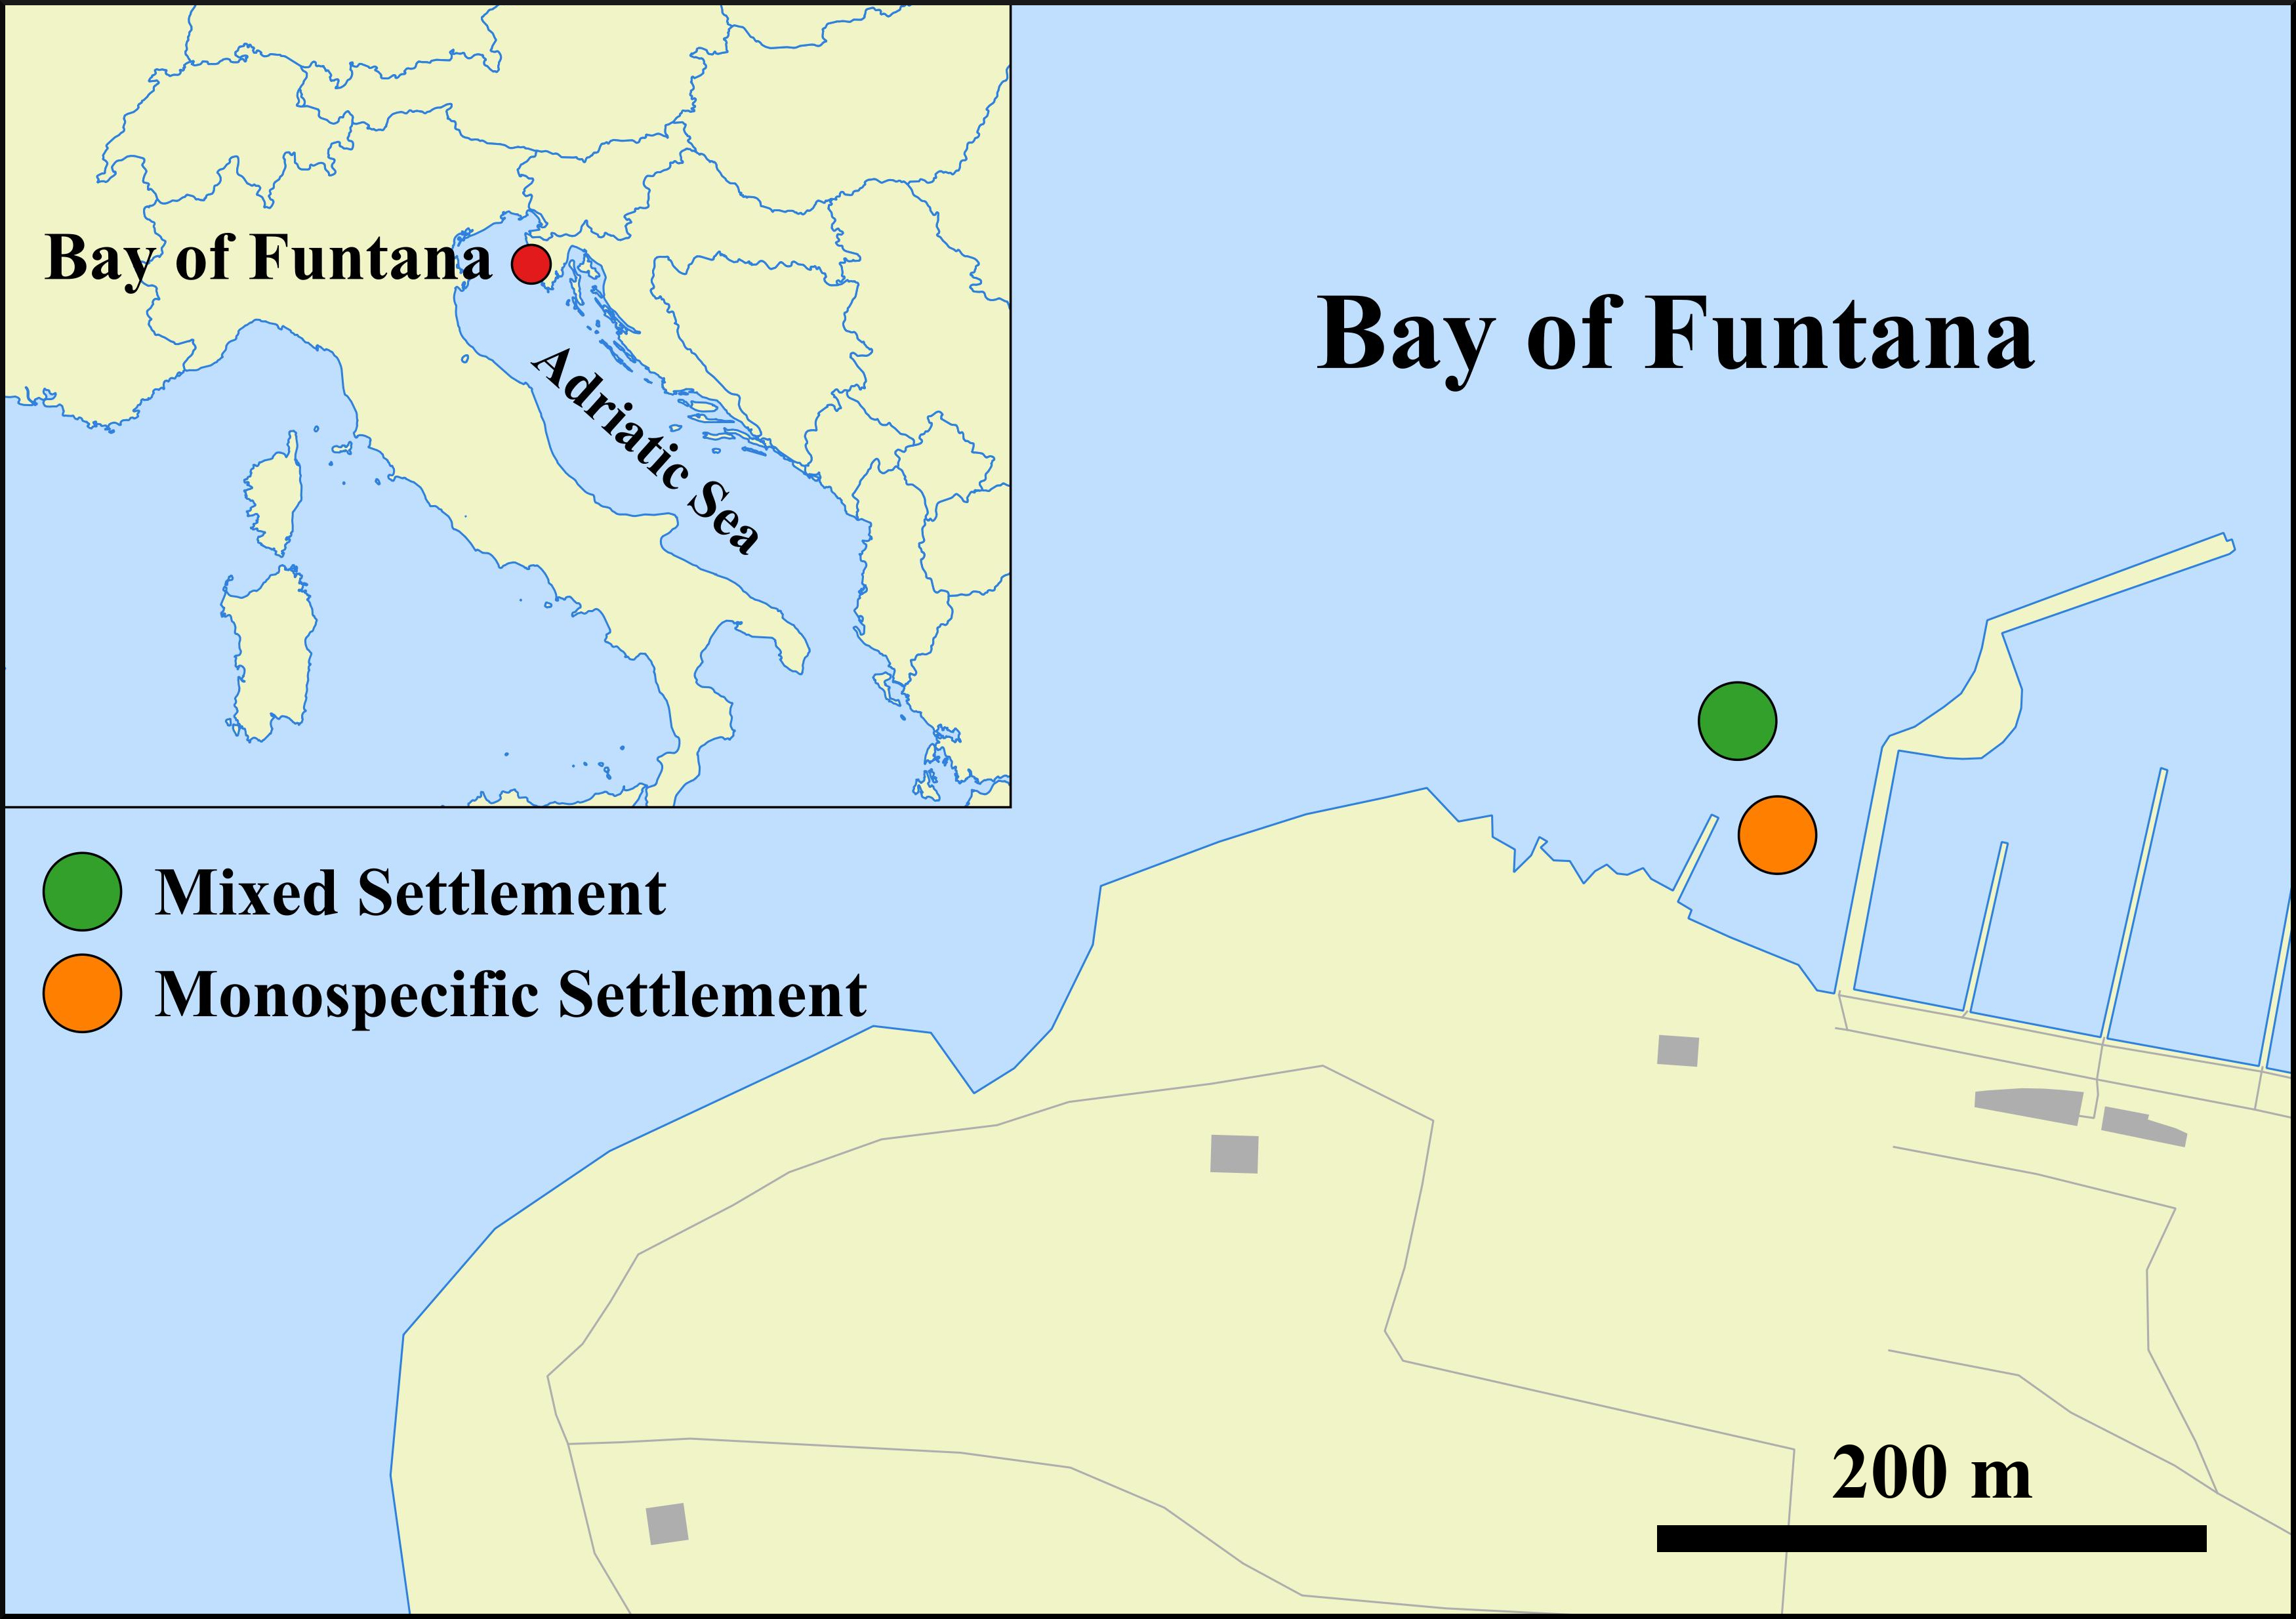
\includegraphics[width=1\linewidth]{/home/marino/Work/repositories/Korlevic_EpiphyticDynamics_FrontMicrobiol_2021/results/figures/map} 

}

\caption{Location of the mixed (\textit{C. nodosa} and \textit{C. cylindracea}) and monospecific (\textit{C. cylindracea}) settlement in the Bay of Funtana, northern Adriatic Sea (© OpenStreetMap contributors, www.openstreetmap.org/copyright).\label{map}}\label{fig:unnamed-chunk-1}
\end{figure}

\begin{figure}[H]

{\centering 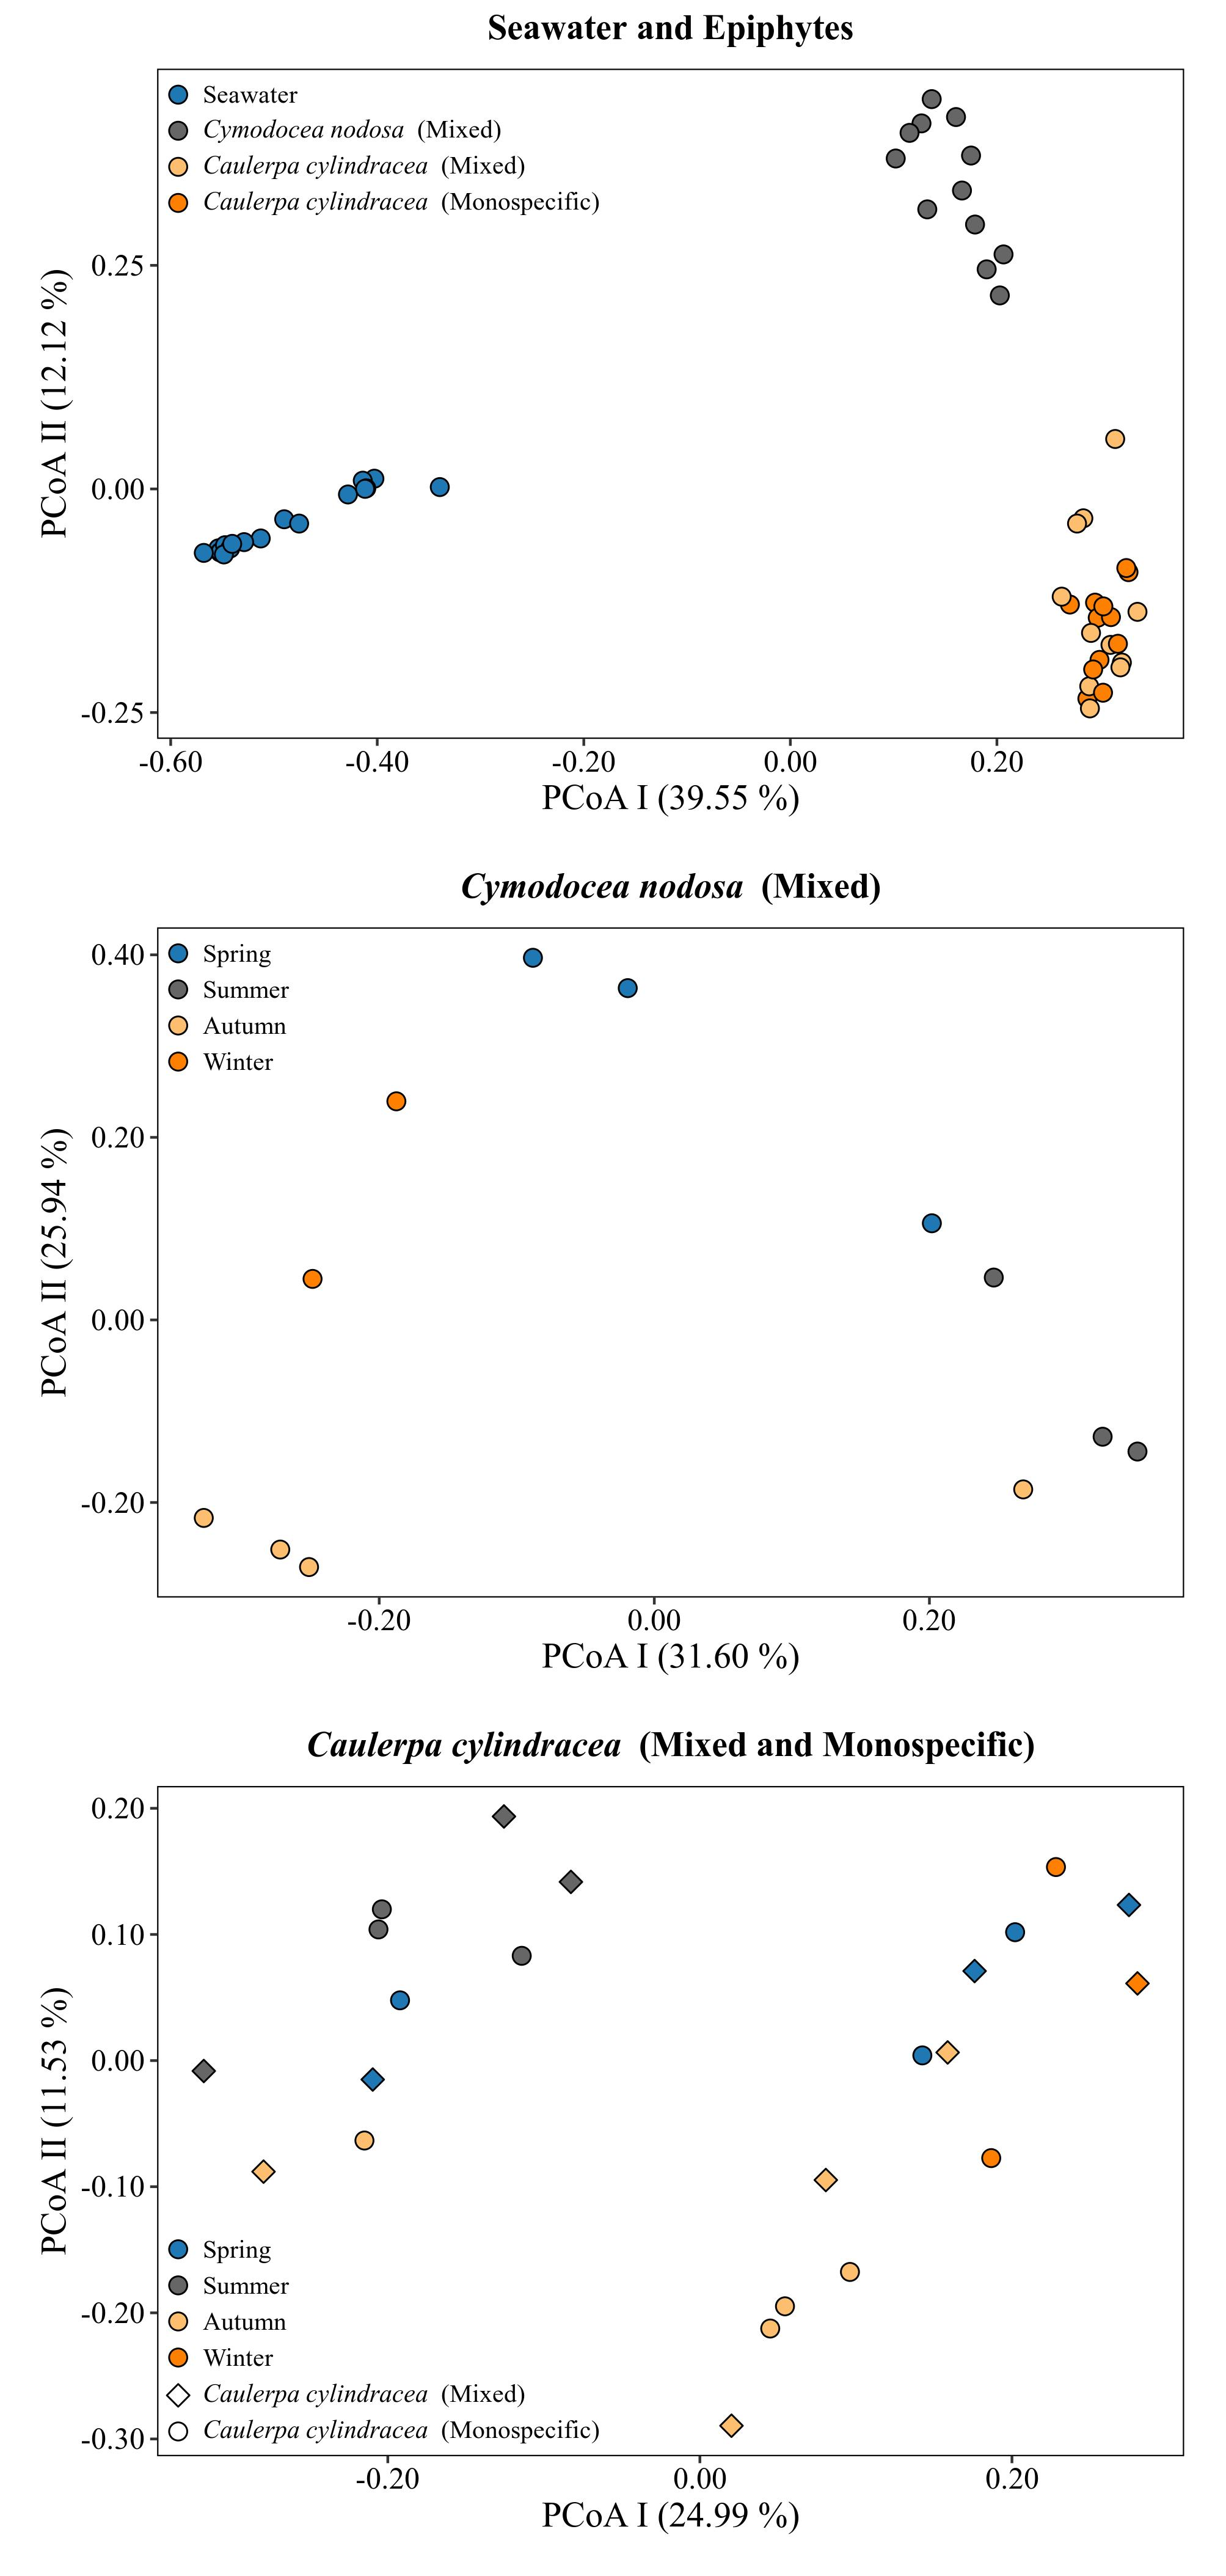
\includegraphics[width=0.55\linewidth]{/home/marino/Work/repositories/Korlevic_EpiphyticDynamics_FrontMicrobiol_2021/results/figures/pcoa_figure} 

}

\caption{Principal Coordinates Analysis (PCoA) of Bray-Curtis distances based on OTU abundances of bacterial and archaeal communities from the surfaces of the macrophytes \textit{C. nodosa} (mixed settlement) and \textit{C. cylindracea} (mixed and monospecific settlement) and in the ambient seawater. Samples from different environments or seasons are labeled in different color and shape. The proportion of explained variation by each axis is shown on the corresponding axis in parentheses.\label{pcoa}}\label{fig:unnamed-chunk-2}
\end{figure}

\begin{figure}[H]

{\centering 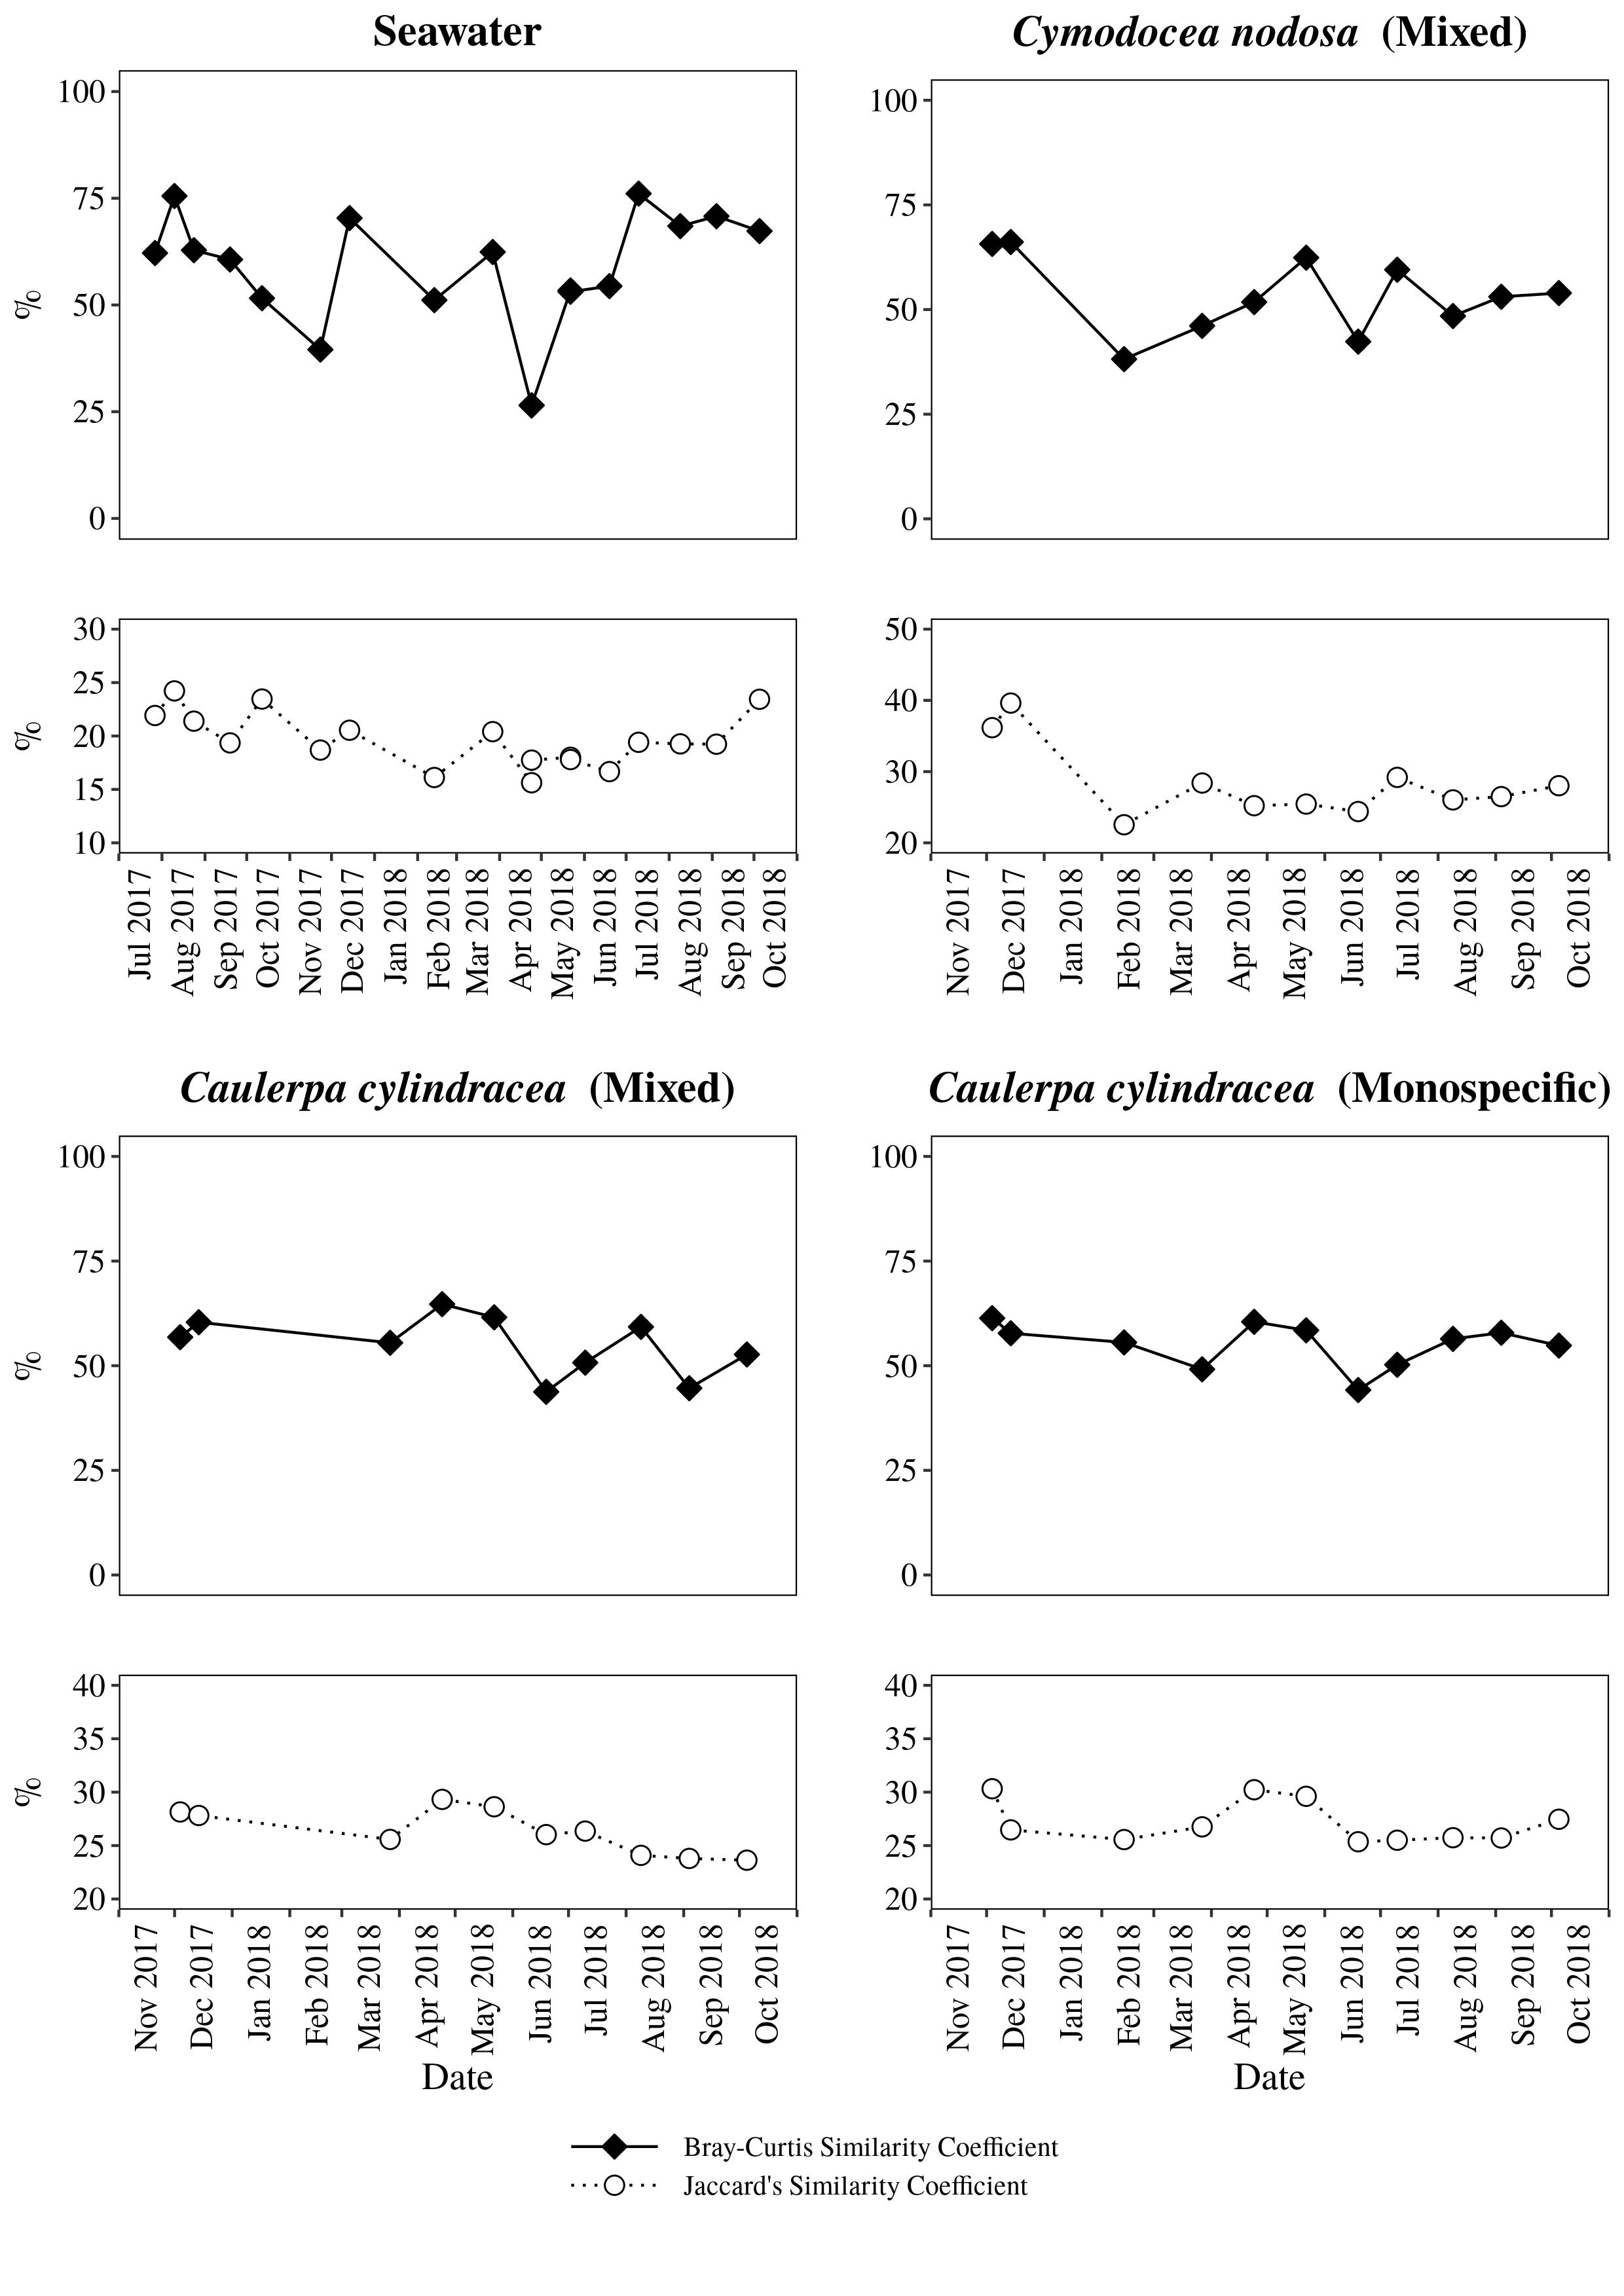
\includegraphics[width=1\linewidth]{/home/marino/Work/repositories/Korlevic_EpiphyticDynamics_FrontMicrobiol_2021/results/figures/seasonal_shared} 

}

\caption{Proportion of shared bacterial and archaeal communities (Bray-Curtis similarity coefficient) and shared bacterial and archaeal OTUs (Jaccard's similarity coefficient) between consecutive sampling dates and from the surfaces of the macrophytes \textit{C. nodosa} (mixed settlement) and \textit{C. cylindracea} (mixed and monospecific settlement) and in the ambient seawater.\label{shared}}\label{fig:unnamed-chunk-3}
\end{figure}

\begin{figure}[H]

{\centering \includegraphics[width=0.85\linewidth]{/home/marino/Work/repositories/Korlevic_EpiphyticDynamics_FrontMicrobiol_2021/results/figures/community_bar_plot} 

}

\caption{Taxonomic classification and relative contribution of the most abundant ($\geq$ 1 \si{\percent}) bacterial and archaeal sequences on the surfaces of the macrophytes \textit{C. nodosa} (mixed settlement) and \textit{C. cylindracea} (mixed and monospecific settlement) and in the ambient seawater. NR -- No Relative (sequences without known relatives within the corresponding group)\label{community}}\label{fig:unnamed-chunk-4}
\end{figure}

\begin{figure}[H]

{\centering \includegraphics[width=0.85\linewidth]{/home/marino/Work/repositories/Korlevic_EpiphyticDynamics_FrontMicrobiol_2021/results/figures/cyanobacteria_bar_plot} 

}

\caption{Taxonomic classification and relative contribution of the most abundant ($\geq$ 1 \si{\percent}) cyanobacterial sequences on the surfaces of the macrophytes \textit{C. nodosa} (mixed settlement) and \textit{C. cylindracea} (mixed and monospecific settlement) and in the ambient seawater. The proportion of cyanobacterial sequences in the total bacterial and archaeal community is given above the corresponding bar. NR -- No Relative (sequences without known relatives within the corresponding group)\label{cyano}}\label{fig:unnamed-chunk-5}
\end{figure}

\begin{figure}[H]

{\centering \includegraphics[width=0.85\linewidth]{/home/marino/Work/repositories/Korlevic_EpiphyticDynamics_FrontMicrobiol_2021/results/figures/bacteroidota_bar_plot} 

}

\caption{Taxonomic classification and relative contribution of the most abundant ($\geq$ 2 \si{\percent}) sequences within the \textit{Bacteroidota} on the surfaces of the macrophytes \textit{C. nodosa} (mixed settlement) and \textit{C. cylindracea} (mixed and monospecific settlement) and in the ambient seawater. The proportion of sequences classified as \textit{Bacteroidota} in the total bacterial and archaeal community is given above the corresponding bar. NR -- No Relative (sequences without known relatives within the corresponding group)\label{bactero}}\label{fig:unnamed-chunk-6}
\end{figure}

\begin{figure}[H]

{\centering \includegraphics[width=0.85\linewidth]{/home/marino/Work/repositories/Korlevic_EpiphyticDynamics_FrontMicrobiol_2021/results/figures/alphaproteobacteria_bar_plot} 

}

\caption{Taxonomic classification and relative contribution of the most abundant ($\geq$ 2 \si{\percent}) alphaproteobacterial sequences on the surfaces of the macrophytes \textit{C. nodosa} (mixed settlement) and \textit{C. cylindracea} (mixed and monospecific settlement) and in the ambient seawater. The proportion of alphaproteobacterial sequences in the total bacterial and archaeal community is given above the corresponding bar. NR -- No Relative (sequences without known relatives within the corresponding group)\label{alpha}}\label{fig:unnamed-chunk-7}
\end{figure}

\begin{figure}[H]

{\centering \includegraphics[width=0.85\linewidth]{/home/marino/Work/repositories/Korlevic_EpiphyticDynamics_FrontMicrobiol_2021/results/figures/gammaproteobacteria_bar_plot} 

}

\caption{Taxonomic classification and relative contribution of the most abundant ($\geq$ 1 \si{\percent}) gammaproteobacterial sequences on the surfaces of the macrophytes \textit{C. nodosa} (mixed settlement) and \textit{C. cylindracea} (mixed and monospecific settlement) and in the ambient seawater. The proportion of gammaproteobacterial sequences in the total bacterial and archaeal community is given above the corresponding bar. NR -- No Relative (sequences without known relatives within the corresponding group)\label{gamma}}\label{fig:unnamed-chunk-8}
\end{figure}

\begin{figure}[H]

{\centering \includegraphics[width=0.85\linewidth]{/home/marino/Work/repositories/Korlevic_EpiphyticDynamics_FrontMicrobiol_2021/results/figures/desulfobacterota_bar_plot} 

}

\caption{Taxonomic classification and relative contribution of the most abundant ($\geq$ 1 \si{\percent}) sequences within the \textit{Desulfobacterota} on the surfaces of the macrophytes \textit{C. nodosa} (mixed settlement) and \textit{C. cylindracea} (mixed and monospecific settlement) and in the ambient seawater. The proportion of sequences classified as \textit{Desulfobacterota} in the total bacterial and archaeal community is given above the corresponding bar. NR -- No Relative (sequences without known relatives within the corresponding group)\label{desulfo}}\label{fig:unnamed-chunk-9}
\end{figure}

\end{document}
